%\documentstyle[graphicx,a4paper,amsmath,amssymb,12pt,oneside,openany,sotsuron,cases,jsreport]{jsbook}
\documentclass[a4paper,12pt,oneside,openany]{jsbook}
\usepackage[dvipdfmx]{graphicx}
\usepackage{graphics}
\usepackage{amsmath}
\usepackage{amssymb}
\usepackage{siunitx}
\usepackage{cases}
\usepackage{jsreport}
\usepackage{sotsuron}
\usepackage{url}
\renewcommand\UrlFont{\rmfamily}
\usepackage{cite}
\usepackage{caption}%基本命令なので入れておく
\usepackage{subcaption}
\usepackage{comment}%複数行,コメントアウトしたいときに使用
\captionsetup{compatibility=false}%これないとエラー出る
\captionsetup[subfigure]{labelformat=simple}
\renewcommand*{\thesubfigure}{(\alph{subfigure})}%subcaptionカッコつける
%\AtBeginDvi{\special{papersize=4AL}}y
%パッケージmathcomp $\tccelsius$で℃使用可
%\newcommand{\bm}[1]{\;\mbox{\boldmath$ {\it #1}$}}
%\newcommand{\mbf}[1]{\mbox{\boldmath$#1$}}
%\newcounter{ass}
%kimura2005/01/14
%\setlength{\cybaseylineskip}{.94\baselineskip}
%行間隔を変える命令<1で狭く,>1で広くする
%\def\baselinestretch{1}
%\pagestyle{empty}	%ページ番号なし
%↓\os{}で上付き文字を使用するための言宣
\newcommand{\os}[1]{\mbox{}^{#1}}
%\bm{}で数式文字太字を使用するための宣言
\newcommand{\bm}[1]{\mbox{\boldmath $#1$}}
\renewcommand{\bibname}{参考文献}	%jsbookの引用文献を参考文献に変える
\newcounter{point}
%自分で入れたやつ

\newcommand{\argmax}{\mathop{arg~max}\limits}
\newcommand{\argmin}{\mathop{arg~min}\limits}

% |\floatsep| は,ページ上部あるいは下部のフロートy間の距離です.
% |\textfloatsep| は,ページ上部あるいは下部のフロートと本文との距離です.
% |\intextsep| は,本文の途中に出力されるフロートと本文との距離です.
% 各基本設定は12pt(多分)

\setlength{\floatsep}{3pt}
\setlength{\textfloatsep}{6pt}
\setlength{\intextsep}{3pt}

%%%%%%%%%%%%%%%%%%%%%%%%%%%%%%%%%%%%%%%%%%%%%%%%%%%%%%%%%%%%%%%%%%%%%%%

\begin{document}
%
%前書き
\frontmatter
%
%タイトル
\title{
\vspace*{-3cm}
{\Large 令和2年度 卒業研究報告書}
\vspace{1cm} \\
 {\Large 題目} \\
{\LARGE \bf 不安定物体を協調支持・搬送可能な\\群ロボット:CarryBotsの開発}\\
\vspace{2.5cm}
 }
\author{
指導教員 \vspace{0.1cm} \\
{\Large 大須賀 公一 教授} \\
{\Large 杉本 靖博 准教授} \\
{\Large 末岡 裕一郎 助教} \\
\vspace{1cm}\\
{\Large 大阪大学 工学部 応用理工学科}\\
  {\Large 学籍番号 08B19704}
  \vspace{0.5cm} \\
  {\LARGE YONG WEI JIE}
\vspace{1.5cm}
}
\date{
{\Large 2021年2月12日}
}
\maketitle

%\thispagestyle{empty}
%\baselineskip 1.15\baselineskip

%概要
\section*{\LARGE 概要}
近年,複数の移動ロボットから構成される群ロボットシステムの研究が進められている.このシステムではロボット同士の協調運搬により,ロボット単体では運搬することができない物体や,複雑な形の物体や,狭いスペースでの物体の運搬などをより効率的な運搬作業を行うことができる.
本研究では,不安定物体を協調支持・搬送可能な群ロボットシステムを提案する.
一般的に,群ロボットによる協調運搬は,各ロボットがグリッパなどの把持機構を利用して,対象物体を掴んで運搬する方法や,単純にロボット自身を使用し,物体を押す方法がある.
これまで開発されてきた協調運搬可能な群ロボットシステムでは安定な物体を主に扱っていたが,本研究の提案するシステムではロボットが対象物体の重心付近まで乗り上げることで,不安定物体でも支持して,運搬することが可能である.
本論文では,不安定物体を支持するための条件を検討する.それをもとに,ロボット同士に乗り上げられる実機システムの設計を行い,実機実験を通じてその妥当性を検証する.


\newpage
%
%目次
\tableofcontents
\newpage
\listoffigures
\newpage
%
%本文
\mainmatter

%内容
\chapter{緒言}
\labsec{introduction}
\section{研究背景および目的}
\labsec{background}
\label{緒言}
近年,複数の移動ロボットから構成される群ロボットシステム(Swarm Robotic Systems)の研究が進められている~\cite{multiRobotCoodination}.複数のロボットが協調して行動することにより,単一のロボットだけでは達成できないような作業を行ったり,より効率的に作業を処理したりすることが可能となる~\cite{swarm}.群ロボットには頑強性(robustness),柔軟性(flexibility),拡張性(scalability)という特徴が求められる.これらの特徴の意味は次のように書ける~\cite{swarmBehaviour}.
\begin{itemize}
 \item 頑強性:群の一部の個体が欠落しても群れ全体の機能を損なわない
 \item 柔軟性:環境が変化したりタスクが変更になったとしてもそれらに適応してタスクを遂行できる
 \item 拡張性:群れの規模が大きくなっても群れ全体の機能が破綻しない
\end{itemize}
これらの特徴を活かした群ロボットのタスクとして,環境センシングやモニタリング~\cite{sensing,monitoring},物体搬送~\cite{motionPlanning}などがあり,さまざまな研究が進められている~\cite{mrs}.その中で,本研究では群ロボットによる協調運搬に着目する.

群ロボットの協調運搬の方式は掴む方法~\cite{grasp1,grasp2,grasp3,swarmBot},押す方法~\cite{push-only1,push-only2,push-only3,argos},囲む方法~\cite{caging1,caging2,caging3}の大きく3つに分類される.
掴む方法を使用する研究として,Dorigoらの「Swarm-bots」と呼ばれるロボット群がある.各ロボットに2本指で挟むグリッパの把持機構が搭載されている.対象物体を認識し,把持機構をうまく操ることで力の相互作用による協調運搬を実現している~\cite{swarmBot}.
また,押す方法を使用する研究として,藤澤らの「ARGOS01」と呼ばれる把持機構なしのゴールや物体を認識できるロボット群がある.蟻の群行動模したフェロモン・コミュニケーションによる他個体誘引および押すことによる餌を蟻の巣に模した場所までの協調運搬を実現している~\cite{argos}.
そして,囲む方法を使用する研究として,WangらのLeader-Follower型のアルゴリズムに基づく制御を行う群ロボットがある.Leader-Follower型の制御系とは移動ロボット群のうち1台をLeader,残りをFollowerと区別し機能分化されたものである.この研究ではLeaderロボットのみに移動軌跡を与え物体を押す.一方,物体を囲むFollowerロボットが物体からの反力・モーメントに基づきその移動軌跡を推定し,協調運搬を実現している~\cite{caging1}.
このうち掴む方法は押す方法と囲む方法と比べて対象物体を2本指で挟むグリッパなどの機構によって掴むことでより安定に協調運搬を実現できる.しかし,対象物体を認識し判断すること,それに合わせた把持動作を考慮すること,把持状態の維持することなどを行うための制御が必要である.
さらに,物体の形によって把持機構ごとに得意不得意が分かれるので,あらゆる形状の物体の把持には至っていない.
それに対して,押す方法と囲む方法は,複雑な把持機構なしで協調運搬を実現できる.
しかし,従来の押す方法と囲む方法には未解決の課題がある.それは倒れやすい不安定な物体の運搬である.

そこで,ロボットが積み上がることで対象物体の重心付近を支持可能な群ロボットシステムは,複雑な把持機構なしで倒れやすい不安定な物体を運搬する良い解決案になるのではないかと考えた.
これを実現するために,ロボット群を対象物体を支持する支持部と全体を移動する移動部に適宜に入れ替われる.対象物体の重心付近を支持するために,支持部は他のロボットに乗り上げられるようなロボットを提案する.すなわち,ロボットが積み上がることより,重心が高い不安定な物体でも支持することができると考えられる.しかし,ロボットの台数に制限があるため,支持部のロボット台数が多いほどより安定な運搬が行うことができる.その一方で,移動部の台数が少なくなり,移動部のロボットに大きな負担をかけるため,協調運搬の効率が悪くなる.したがって,効率よく協調運搬する群ロボットシステムを実現するために,物体の形や運搬速度などの条件に応じて,移動部と支持部の割合を適切に設計することが望ましい.

よって,本研究では,\reffig{proposed-system}に示すように,ロボットが対象物体の重心付近まで乗り上げることにより,ロボット自身の体を活用して物体を支持し,あらゆる形状の物体の協調運搬を実現する群ロボットシステムを提案する.
\begin{figure}[tb]
  \centering
  \includegraphics[width=0.96\columnwidth]{figure/proposed-system.pdf}
  \caption{Proposed system}
  \label{fig:proposed-system}
\end{figure}
% \begin{figure}[bt]
%   \vspace{6mm}
%   \centering
%   \begin{tabular}{c}
%     \begin{minipage}[ht]{0.33\columnwidth}
%       \centering
%       \includegraphics[trim=0 0 0 0, clip,width=\columnwidth]{./figure/unstable3.jpeg}
%     %   \subcaption{Unstable1}
%       \labfig{Unstable1}
%     \end{minipage}
%     \begin{minipage}[ht]{0.33\columnwidth}
%       \centering
%       \includegraphics[trim=0 0 0 0, clip,width=\columnwidth]{./figure/unstable2.jpeg}
%     %   \subcaption{Unstable2}
%       \labfig{Unstable2}
%     \end{minipage}
%     \begin{minipage}[ht]{0.33\columnwidth}
%       \centering
%       \includegraphics[trim=0 0 0 0, clip,width=\columnwidth]{./figure/unstable1.jpeg}
%     %   \subcaption{Unstable3}
%       \labfig{Unstable3}
%     \end{minipage}
%   \end{tabular}
%   \centering
%   \caption{Proposed system}
%   \labfig{proposed-system}
% \end{figure}
また,\reffig{tradeoff}では,移動部と支持部の割り当てによって,物体の安定性と全体の機動性の間のトレードオフを示す.
\begin{figure}[bt]
  \vspace{0mm}
  \centering
  \begin{tabular}{c}
    \begin{minipage}[ht]{0.5\columnwidth}
      \centering
      \includegraphics[trim=0 0 0 0, clip,width=\columnwidth]{figure/tradeoff-fast.pdf}
      \subcaption{Supporter: 2, Mover: 18}
      \labfig{tradeoff1}
    \end{minipage}
    \begin{minipage}[ht]{0.5\columnwidth}
      \centering
      \includegraphics[trim=0 0 0 0, clip,width=\columnwidth]{figure/tradeoff-stable.pdf}
      \subcaption{Supporter: 12, Mover: 8}
      \labfig{tradeoff2}
    \end{minipage}
  \end{tabular}
  \centering
  \caption{Tradeoff between stability and mobility}
  \labfig{tradeoff}
\end{figure}
最終目標として,移動部と支持部の最適な割合を設計し,機能を適応的に分化させながら,協調して運搬作業を行うシステムの実現を目指している.すなわち,不安定物体の姿勢を安定させることと効率よく運搬することを両立させる群ロボットシステムの実現を目指している.
本研究では,その前段階として,乗り上げることで対象物体を支持でき,乗り上げたり,降りたりすることによって支持部と移動部の間で切り替えられるロボットを製作する.

それに向けて本論文では,提案システムのモデリングをして,搬送物体をロボットで支持するための条件を検討し,それをもとに実機を製作した.
また,モデリングした式からロボットと物体の高さの比を設計することに注目し,隣接しているロボットに乗り上げられるロボットを製作し,ロボットが積み上がることで,対象物体の支持が可能であることを示す.
さらに,物体の姿勢をロボットにフィードバックし,ロボットの前進力を制御することで,物体をより安定に支持できることを示す.

\section{本論文の構成}
本論文の構成は,以下の通りである.
まず,2章では提案したシステムについて述べる.
次に,3章で開発した不安定物体が支持可能な群ロボットについて述べる.
そして,4章で製作したロボットを用いて実験を行い,実験結果に対する考察について述べる.
最後に,5章で本論文をまとめる.


\chapter{不安定物体を支持可能な群ロボットシステム}
本章では,まず提案する不安定物体を支持可能な群ロボットシステムについて説明する.
次に,システムのモデリングについて説明する.

%--------------------------------------------------------------
\section{システムの提案}
本研究の提案する自身の体で不安定な物体を支持し運搬する群ロボットシステムを実現するために,ロボット群が搬送物体を支持する支持部とシステム全体を移動する移動部に分ける必要がある.

また,ロボットの台数は限られているので,支持部のロボットの台数が多いほど,物体を安定に支持できるが,移動部に負担がかかるため,全体の移動速度が遅くなることが考えられる.一方,移動部に関しては,ロボットが多いほど,全体の速度は速いが,支持部のロボットが少ないため,物体が倒れる可能性がある.

本研究の最終目標として,支持部と移動部の間のトレードオフを考慮し,最適の割合でロボット群にタスクを割り当てる必要がある.今回の研究はその前段階として,支持部のロボットが物体を支えるための条件を検討する.
\section{問題設定}
環境・ロボット・運搬対象物に関する前提条件は以下の通りとする.
\begin{itemize}
    \item 環境
    \begin{itemize}
        \item 平面
    \end{itemize}
    \item ロボット
    \begin{itemize}
        \item 前後移動可能
        \item 物体を両側から支持して運搬する
        \item 支持と移動の役割を分担させる
        
    \end{itemize}
    \item 運搬対象物
    \begin{itemize}
        \item 左右だけに倒れる長方形
        \item 重心位置,物体位置は既知
        \item 初期姿勢からの傾きの許容範囲は±5deg未満
    \end{itemize}
    
\end{itemize}
\section{システム全体のモデル}
\label{section:modeling}
物体が倒れるときや物体を支持するための条件を検討するために,システムのモデリングを行う.そのモデリングの概要について述べる.モデリングした図を\reffig{modeling}に示す.ここで,縦長い物体を真ん中に立てて,その両側に長方形のロボットが置いてある.ロボット1とロボット2は左と右にそれぞれ置く.また,これらを移動部の上に乗せた.今回移動部は地面との摩擦を無視できる横長い台車と仮定し,ロボットと物体の間の抗力は中央に作用すると仮定する.\reffig{freebody}に物体に作用する力の図を示す.ここで,物体に重力による力,ロボットと台車からの垂直抗力,ロボット・台車との摩擦が作用する他に,台車に力をかけた場合の物体にそれと逆向きに慣性力$F^{\prime}$が働く.また,ロボット1とロボット2の寸法は同じなので,$h_{r_1}=h_{r_2}=h_{r}$とする.
本稿におけるモデリングに使用した変数を\reftab{model-parameter}に示す.
\begin{figure}[tb]
  \centering
    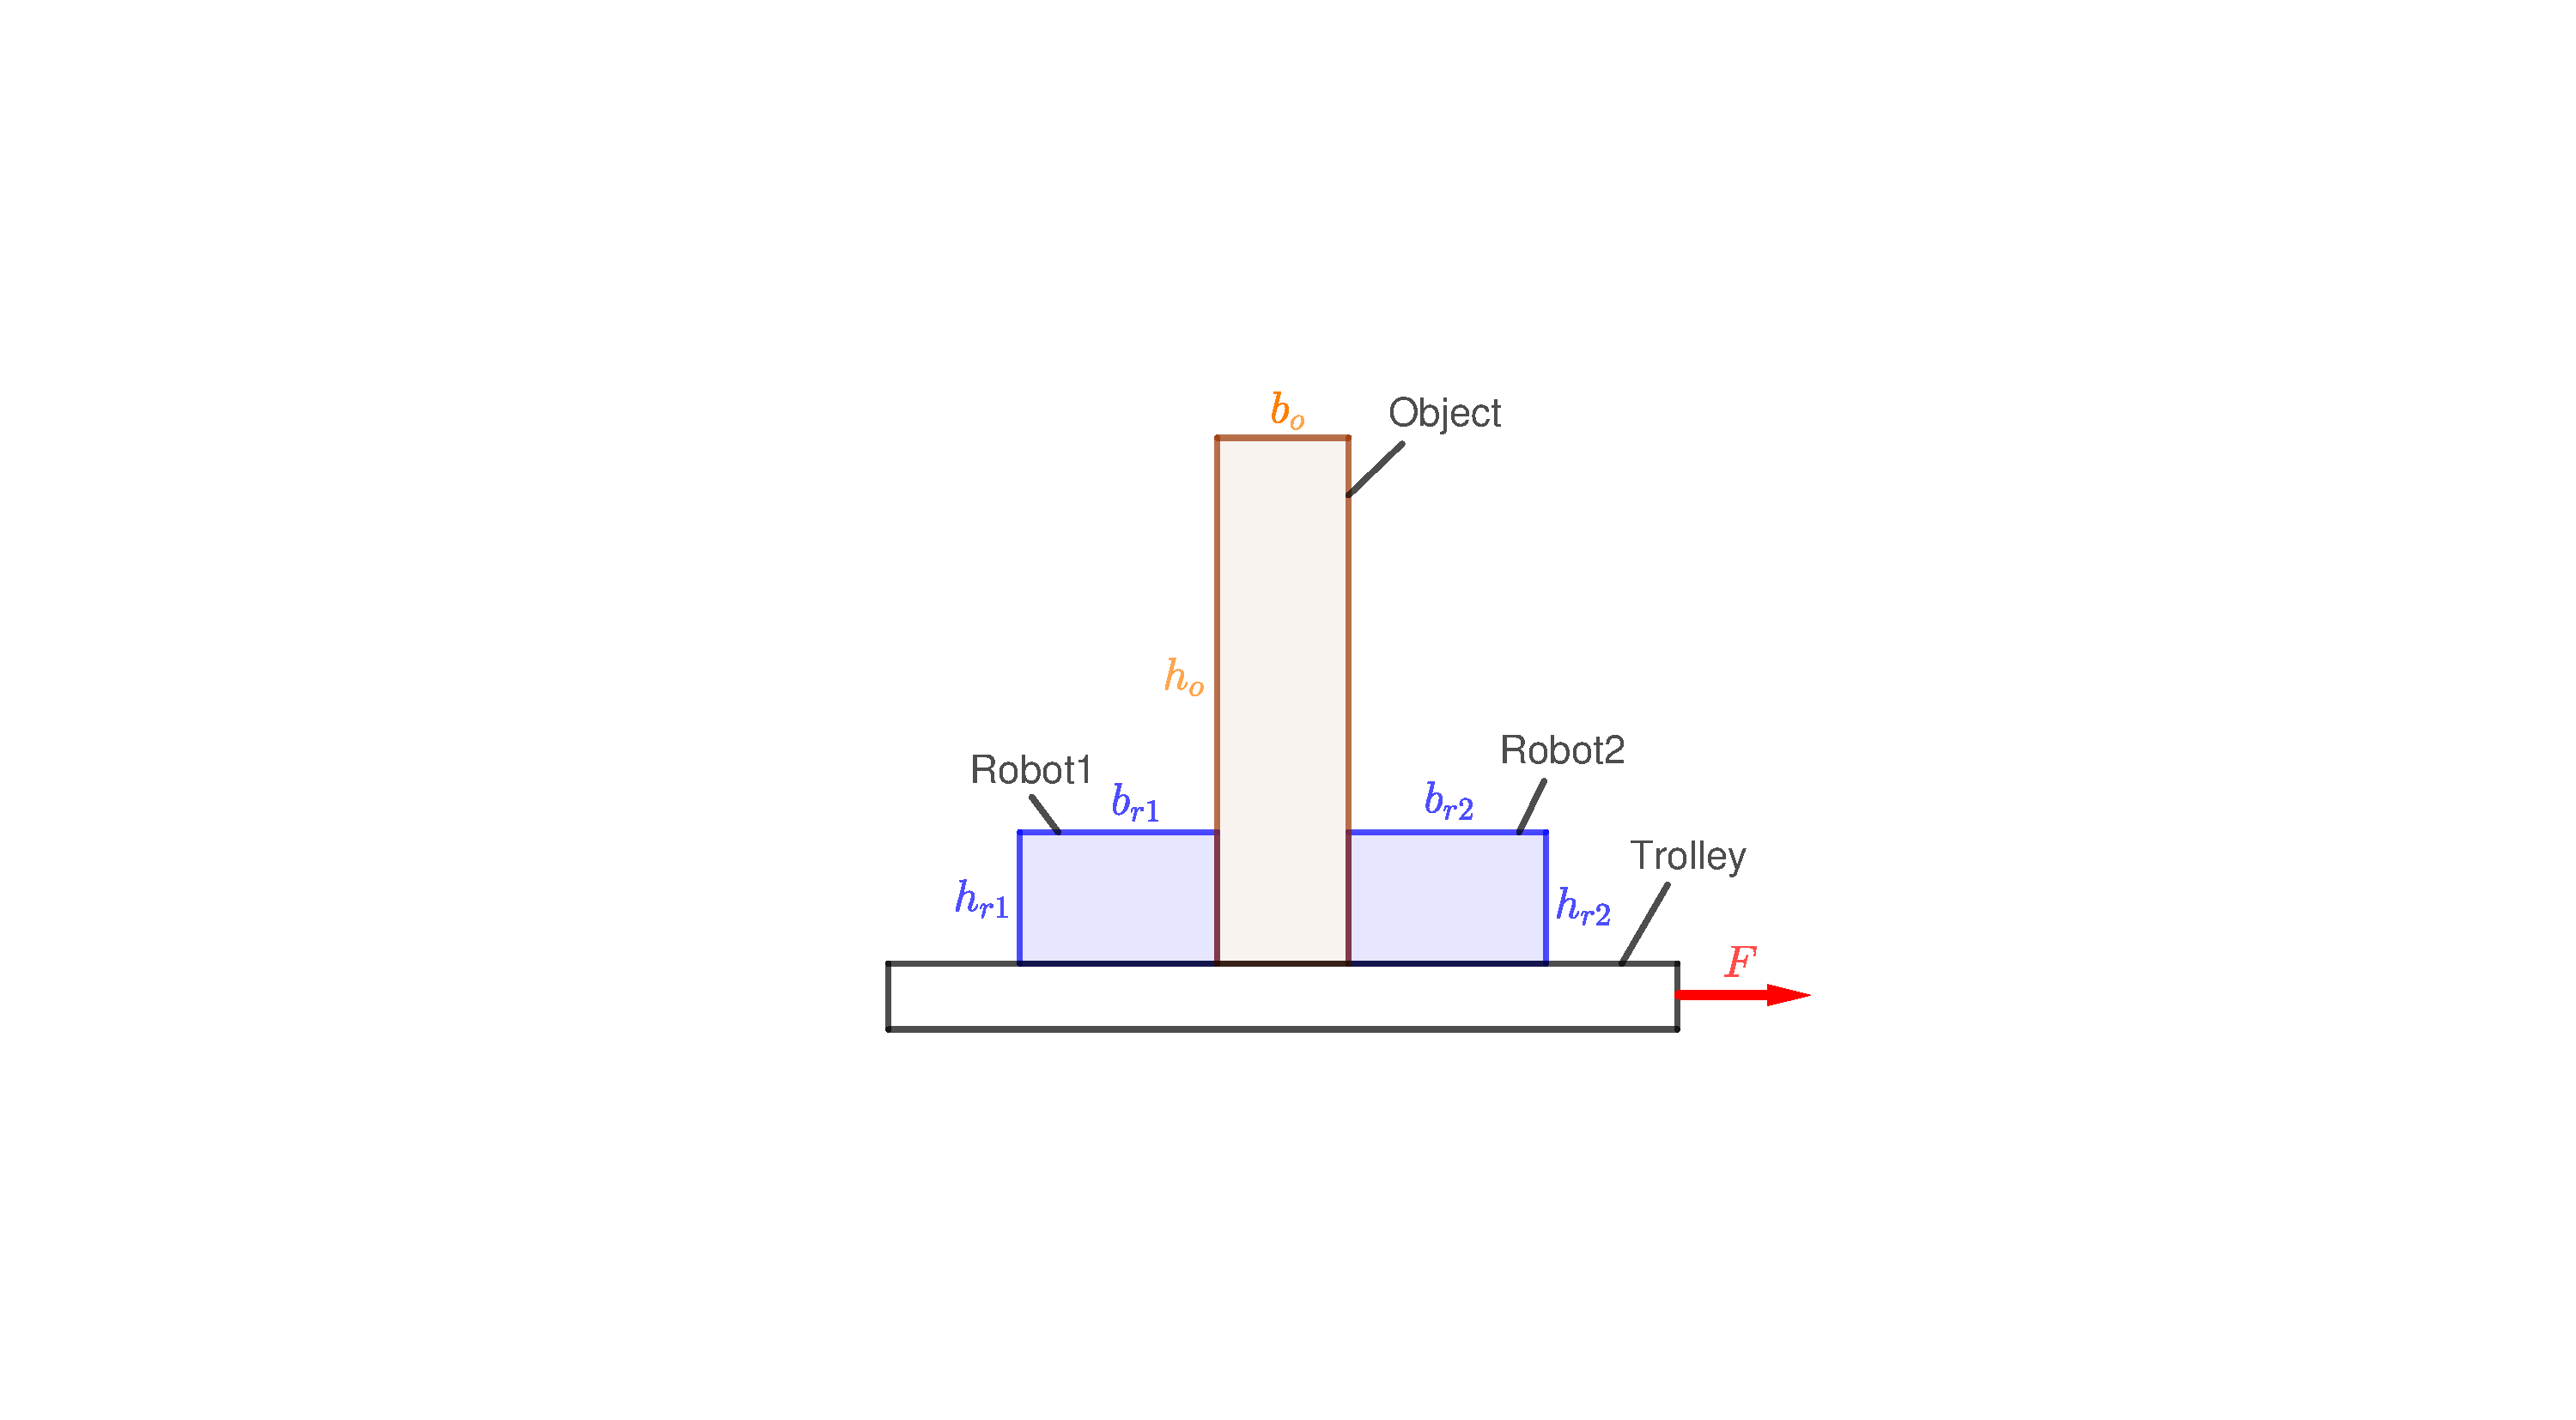
\includegraphics[width=0.65\columnwidth]{./figure/carrybot-model.pdf}
    \caption{Simplified model}
    \labfig{modeling}
\end{figure}
\begin{figure}[tb]
  \centering
    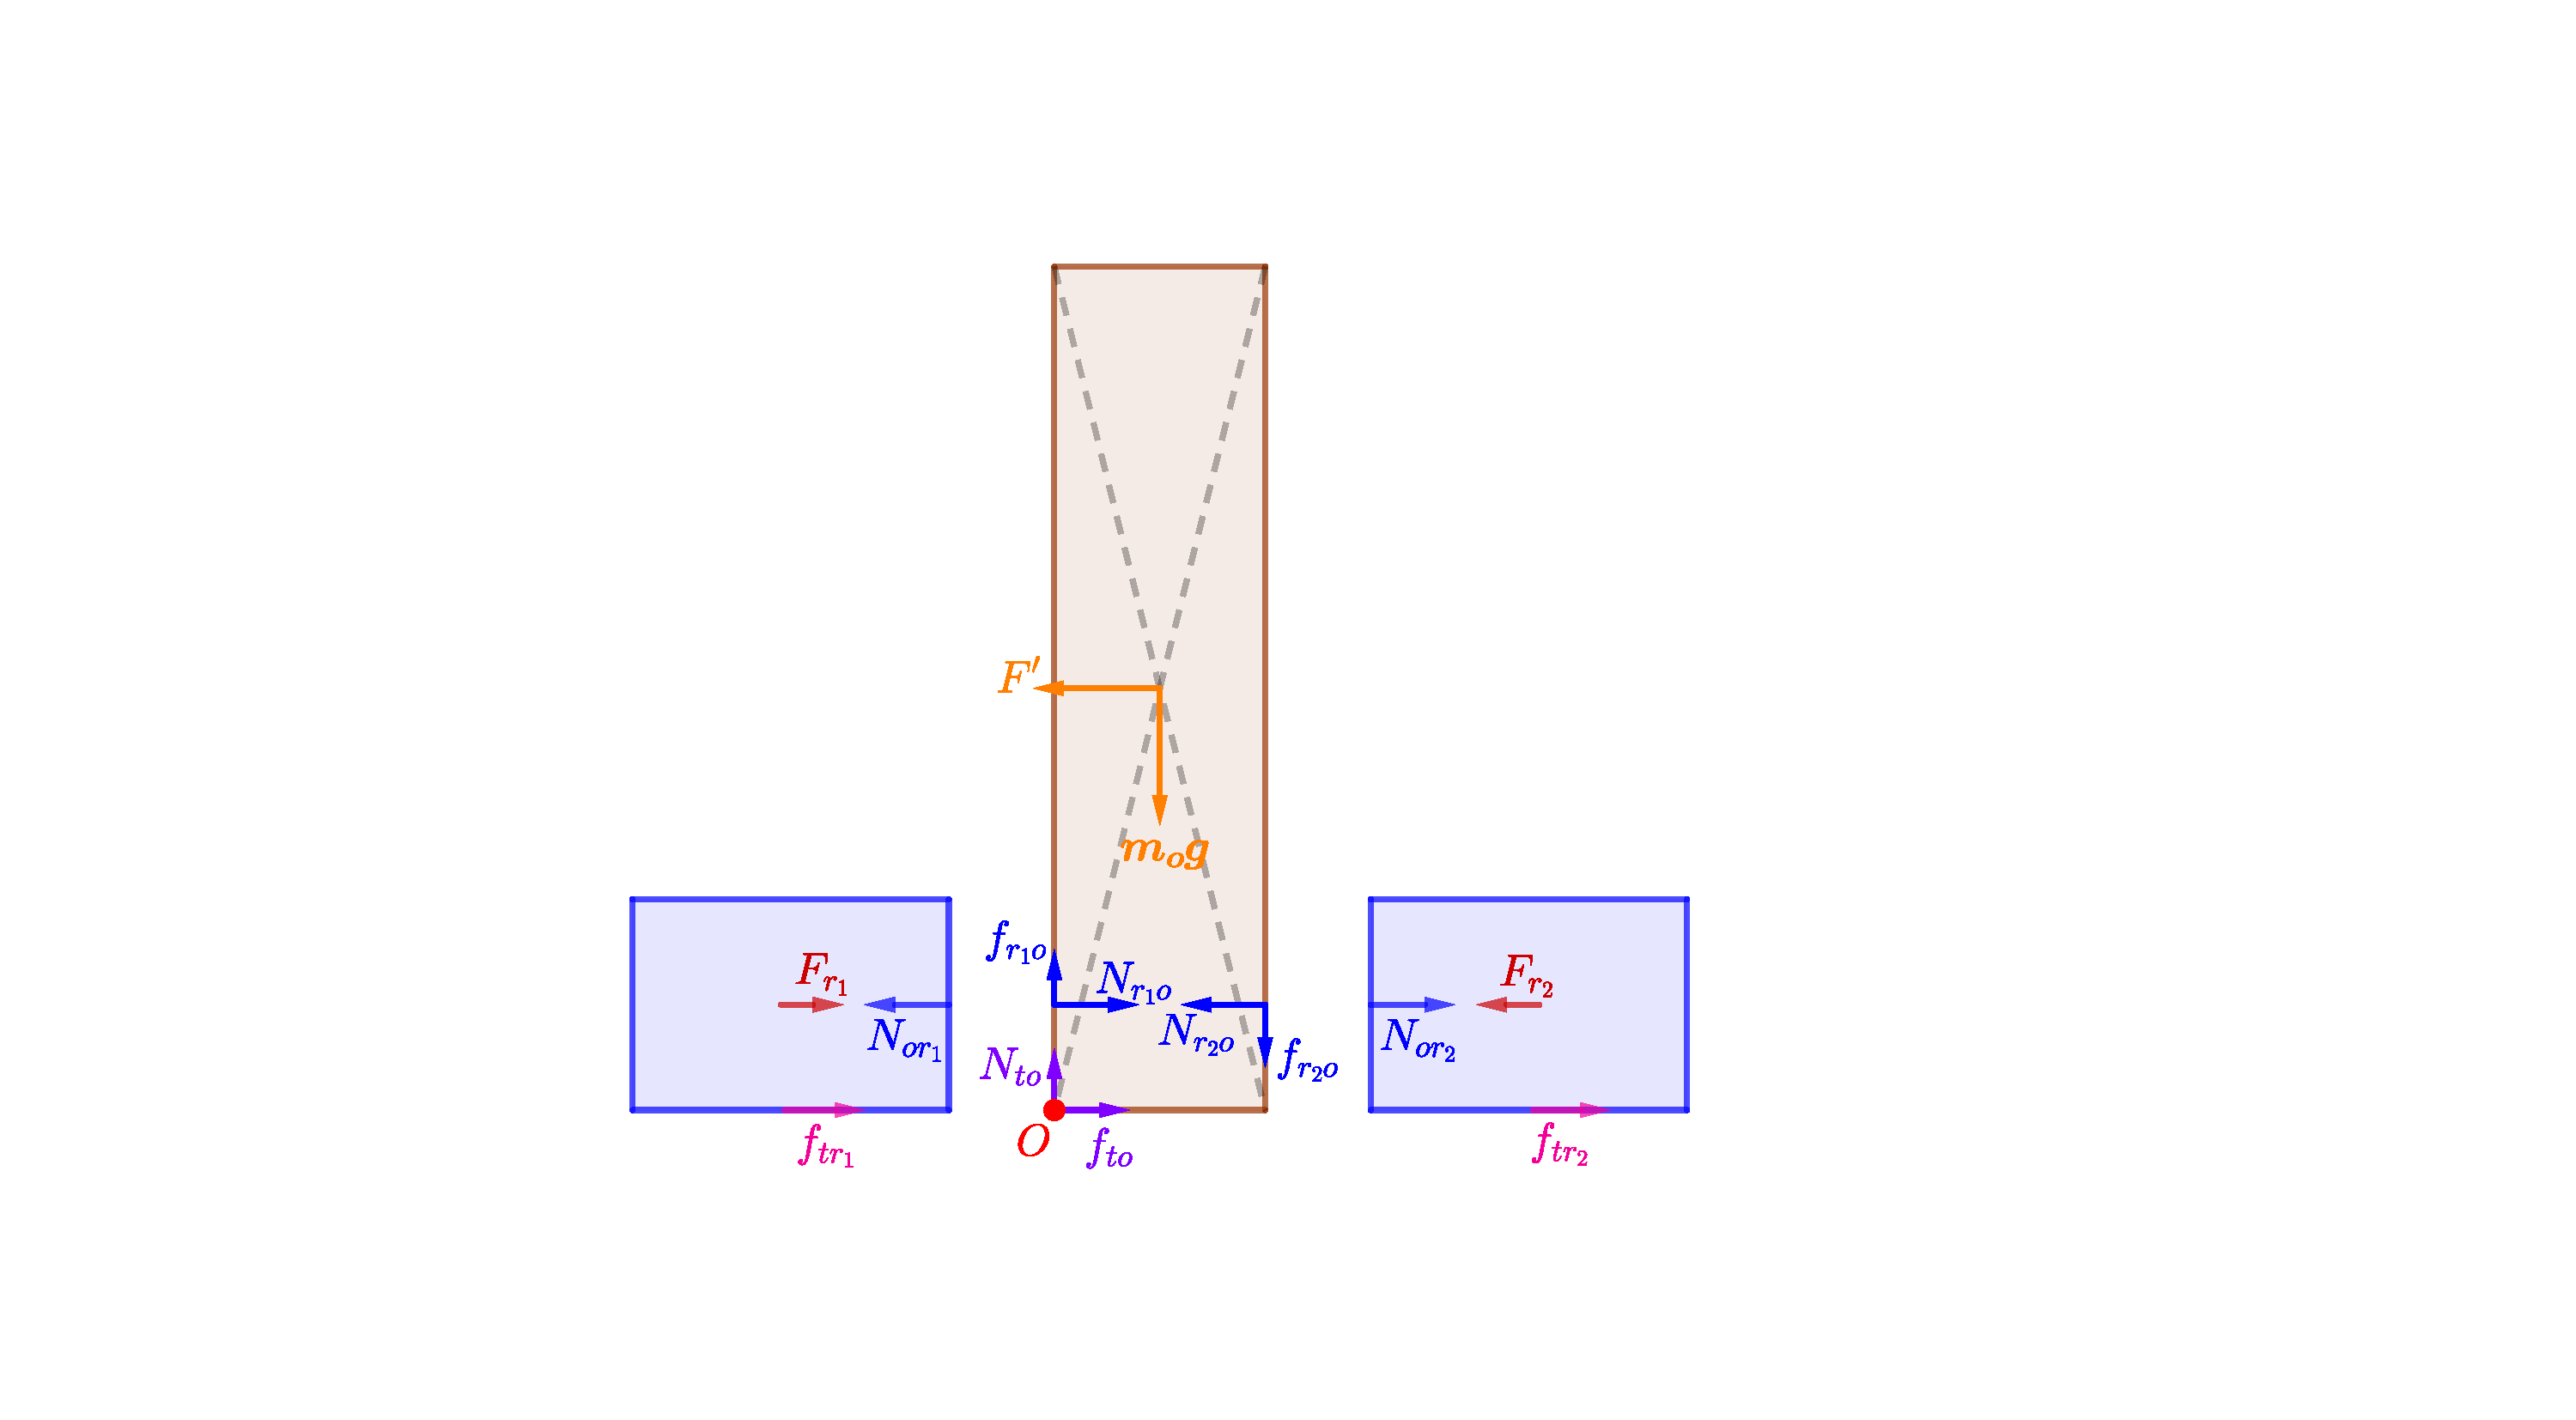
\includegraphics[width=0.65\columnwidth]{./figure/freebody-v2.pdf}
     \caption{Free body diagram of object and robot}
     \labfig{freebody}
\end{figure}

\begin{table}[tb]
\caption{Parameters of model}
\centering
\begin{tabular}{c|c}
\hline
Parameter & Description                   \\ \hline\hline
$b_o$       & Width of object              \\ \hline
$h_o$      & Height of object               \\ \hline
$h_r$      & Height of robot               \\ \hline
$m_o$     & Mass of object        \\ \hline
$f_{r_1 o}$       & Friction from robot1 acting on object                 \\ \hline
$f_{r_2 o}$ & Friction from robot2 acting on object                 \\ \hline
$f_{t o}$ & Friction from trolley acting on object                 \\ \hline
$N_{t o}$ & Normal force from trolley acting on object                 \\ \hline
$N_{r_1 o}$ & Normal force from robot1 acting on object                 \\ \hline
$N_{r_2 o}$ & Normal force from robot2 acting on object                 \\ \hline
$F_{r_1}$ & Force asserted by robot1                 \\ \hline
$F_{r_2}$ & Force asserted by robot2                 \\ \hline
\end{tabular}
\label{tab:model-parameter}
\end{table}

次に,物体が傾き始めるの台車にかけるための右向きの力を調べる.ここで,物体が傾き始める条件は台車からの垂直抗力の作用点と回転軸の一致である.この条件のもとに,\reffig{freebody}に示すような物体に働く内力についての点$O$まわりのモーメントを考える.ここで,右まわりのモーメントが左まわりのモーメントより大きいとき,物体が倒れない.つまり,\eqref{equilibrium}式が成り立つとよい.
\begin{equation}
F^{\prime} \frac{h_{o}}{2}+N_{r_{2} o} \frac{h_{r}}{2}<m_{o} g \frac{b_{o}}{2}+N_{r_{1} o} \frac{h_{r}}{2}+f_{r_{2} o} b_{o}
\label{equilibrium}
\end{equation}
\eqref{equilibrium}式では,左辺に点$O$を中心として左まわりのモーメントを示し,その右辺に右まわりのモーメントを示す.
また,$F^{\prime}$について解き,物体が傾かないための条件が\eqref{F-solve}式である.
\begin{equation}
    F^{\prime}<\frac{h_{r}}{h_{o}}\left(N_{r_{1} o}-N_{r_{2} o}\right)+\frac{b_{o}}{h_{o}}\left(m_{o} g+2 f_{r_2 o}\right)
    \label{F-solve}
\end{equation}
\eqref{F-solve}式より,右辺を大きくするほど,台車に大きな力がかかっても物体は傾かないため,物体をより安定に運ぶことができると考えられる.
よって,\eqref{F-solve}式右辺を大きくすることに着目する.
さらに,\eqref{F-solve}式の右辺の1項目のロボット1からの垂直抗力$N_{r_1 o}$とロボット2からの垂直抗力$N_{r_2 o}$を\reffig{freebody}に示すようなそれぞれのロボットの前進力$F_{r_1}$,$F_{r_2}$,ロボットと台車の間の摩擦力$f_{tr_1}$,$f_{tr_2}$で表現すると,
$N_{r_{1} o}=F_{r_{1}}+f_{t{r_1}}$,
$N_{r_{2} o}=F_{r_{2}}-f_{t{r_2}}$
が得られる.これらを\eqref{F-solve}式に代入すると,
\begin{equation}
    F^{\prime}<\frac{h_{r}}{h_{o}}\left(F_{r_{1}}-F_{r_{2}}+f_{t{r_1}}+f_{t{r_2}}\right)+\frac{b_{o}}{h_{o}}\left(m_{o} g+2 f_{r_2 o}\right)
    \label{F-solve-again}
\end{equation}
になる.
ただし,\reffig{freebody}に示すように物体の左にあるロボット1の前進力$F_{r_{1}}$は右方向に働く.一方,物体の右にあるロボット2の前進力$F_{r_{2}}$は左方向に働く.

以上から,\eqref{F-solve-again}式より,右辺を大きくし,物体をより安定に運べるための条件を以下にまとめる.1項目に関しては,
\begin{enumerate}
    \item ロボットと物体の高さの比$\frac{h_{r}}{h_{o}}$を大きくする.
    \item ロボット1とロボット2の前進力の差$F_{r_{1}}-F_{r_{2}}$を大きくする.
    \item ロボットと台車の間の摩擦$f_{t{r_1}}+f_{t{r_2}}$を大きくする. 
\end{enumerate}
2項目に関しては,
\begin{enumerate}
    \setcounter{enumi}{3}
    \item 物体の幅と高さの比$\frac{b_{o}}{h_{o}}$を大きくする.
    \item 物体の質量$m_{o}$を大きくする.
    \item ロボット2と物体との摩擦$f_{r_2 o}$を大きくする.  
\end{enumerate}
上に述べた条件の中で,4,5は既定で,1,2,3,6が可変なパラメータである.ここで筆者はロボットと台車の間の摩擦に注目した.すなわち,上下のロボット同士の間の摩擦をできるだけ大きくすることを目標に実機の開発を行う.そして,1,2の設計に注目し,3章で作製した実機で4章で検証実験を行う.

% \[
% F_{\text { topple }(O_2)}=\frac{1}{h_{o}-2 h_{r}}\left[h_{r}\left(N_{r_{2} o}-N_{r_{1} o}+2 f_{t o}\right)+b_{o}\left(m_{o} g+2 f_{r_2 o}\right)\right]
% \]

%\section{シミュレーション概要}

\chapter{CarryBotsの機構と開発}
本章では,製作した不安定物体を支持可能な車輪型移動ロボットについて述べる.
まず,提案するピニオン車輪&ラックレール機構について述べる.
次に,物体の姿勢を検知するセンサについて述べる.
そして,製作したロボットについて述べる.

\section{ピニオン車輪&ラックレール機構の提案}
前章で述べた式から,上下のロボット間の摩擦を上げることで,物体をより安定に支持することができることがわかった.そこで,それをできる限り大きくするために,ラック・アンド・ピニオン(rack and pinion)機構を採用した.
ロボットにピニオンのような小口径の円形歯車の形の車輪(以下,ピニオン車輪と表記)を利用し,ロボットの上面に歯がつけられたラックの形をしているレール(以下,ラックレールと表記)をつける.ロボットが乗り上げる際に,乗り上げる側のピニオン車輪が乗り上げられる側のラックレールとかみ合わさることで,ロボットは前後にずれることがほとんどなくなり,上下のロボット間の摩擦は非常に大きくなると言える.その他,このピニオン車輪&ラックレール機構を利用すると,ロボットが斜めにずれることを防ぐという利点や,急勾配を登り下りするための推進力と制動力の補助になるという利点が挙げられる.この構造を用いた車輪の外観を\reffig{rack-pinion-concept}に示す.

しかし,地面にあるロボットはピニオン車輪のままで移動すると,ピニオン車輪の歯と地面の接触面積が少ないため,滑りやすいという問題がある.また,とき間が経つと,地面との摩擦でピニオン車輪の歯の摩耗も考えられる.これらの問題を解決するために,\reffig{pinion-wheel-edited}に示すようにピニオン車輪の歯先に滑りにくい,軟質樹脂製パッドをつけることを考えた.これによって,ピニオン車輪のグリップを高める効果が出すことができると,歯の摩耗も解消できると考えられる.

\begin{figure}[tb]
  \centering
  \includegraphics[width=\columnwidth]{./figure/rack-pinion-v2.pdf}
  \caption{Overview of proposal rack-rail and pinion-wheel}
  \label{fig:rack-pinion-concept}
\end{figure}


\begin{figure}[tb]
  \centering
  \includegraphics[width=.8\columnwidth]{figure/elastomer-insert-v2.pdf}
  \caption{3D model of the pinion-wheel and elastomer insert}
  \label{fig:pinion-wheel-edited}
\end{figure}


\section{物体の姿勢を検知するセンサ}
次に,ロボットが物体の姿勢を検知するためのセンサとして,リミットスイッチを採用した.\reffig{limit-switch-edited}に示すように,リミットスイッチを平行に並べると,スイッチの当たり具合で物体の姿勢が推定できると考えられる.例えば,スイッチが二つ同ときに反応した場合,物体は地面に対して垂直であると判定し,下のスイッチだけ反応したら,物体はロボットと反対側に傾いていると判断することができる.リミットスイッチの間の距離を設計することで,物体の傾きの許容範囲を決定することができる.また,物体の傾きを検知する分解能を上げたい場合には,リミットスイッチを数を増やすことで対応することができる.

\begin{figure}[tb]
  \centering
  \includegraphics[width=.5\columnwidth]{figure/posture-detector-v2.pdf}
  \caption{3D model of the posture detector}
  \label{fig:limit-switch-edited}
\end{figure}

\section{実機製作}
前節で設計したピニオン車輪&ラックレールを用いて開発したロボットの外観を\reffig{carrybot}に示す.ロボットの各種パラメータを\reftab{robot-specs}に示す.本体の白色部分と白色のピニオン車輪は3Dプリンタ(X-Smart Qidi Technology製,X-Maker Qidi Technology製)を使ってPLA樹脂を射出成形したものであり,透明部分はTAMIYA製の透明プラバン$0.4$~mmを切り出したものである.透明プラバンの上につけた白色のラックレールは3Dプリンタを使ってTPU(熱可塑性ポリウレタン)を射出成形したものである.ロボットに搭載したマイコン,モータドライバ,モータ,リミットスイッチおよびバッテリーの詳細を以下に示す.また,それらの外観を\reffig{parts}に示す.

\begin{figure}[ht]
  \vspace{0mm}
  \centering
  \begin{tabular}{c}
    \begin{minipage}[ht]{0.5\columnwidth}
      \centering
      \includegraphics[width=\columnwidth]{figure/carrybot-diagonal.pdf}
      \subcaption{Diagonal view}
      \labfig{diagonal-view}
    \end{minipage}
    \begin{minipage}[ht]{0.5\columnwidth}
      \centering
      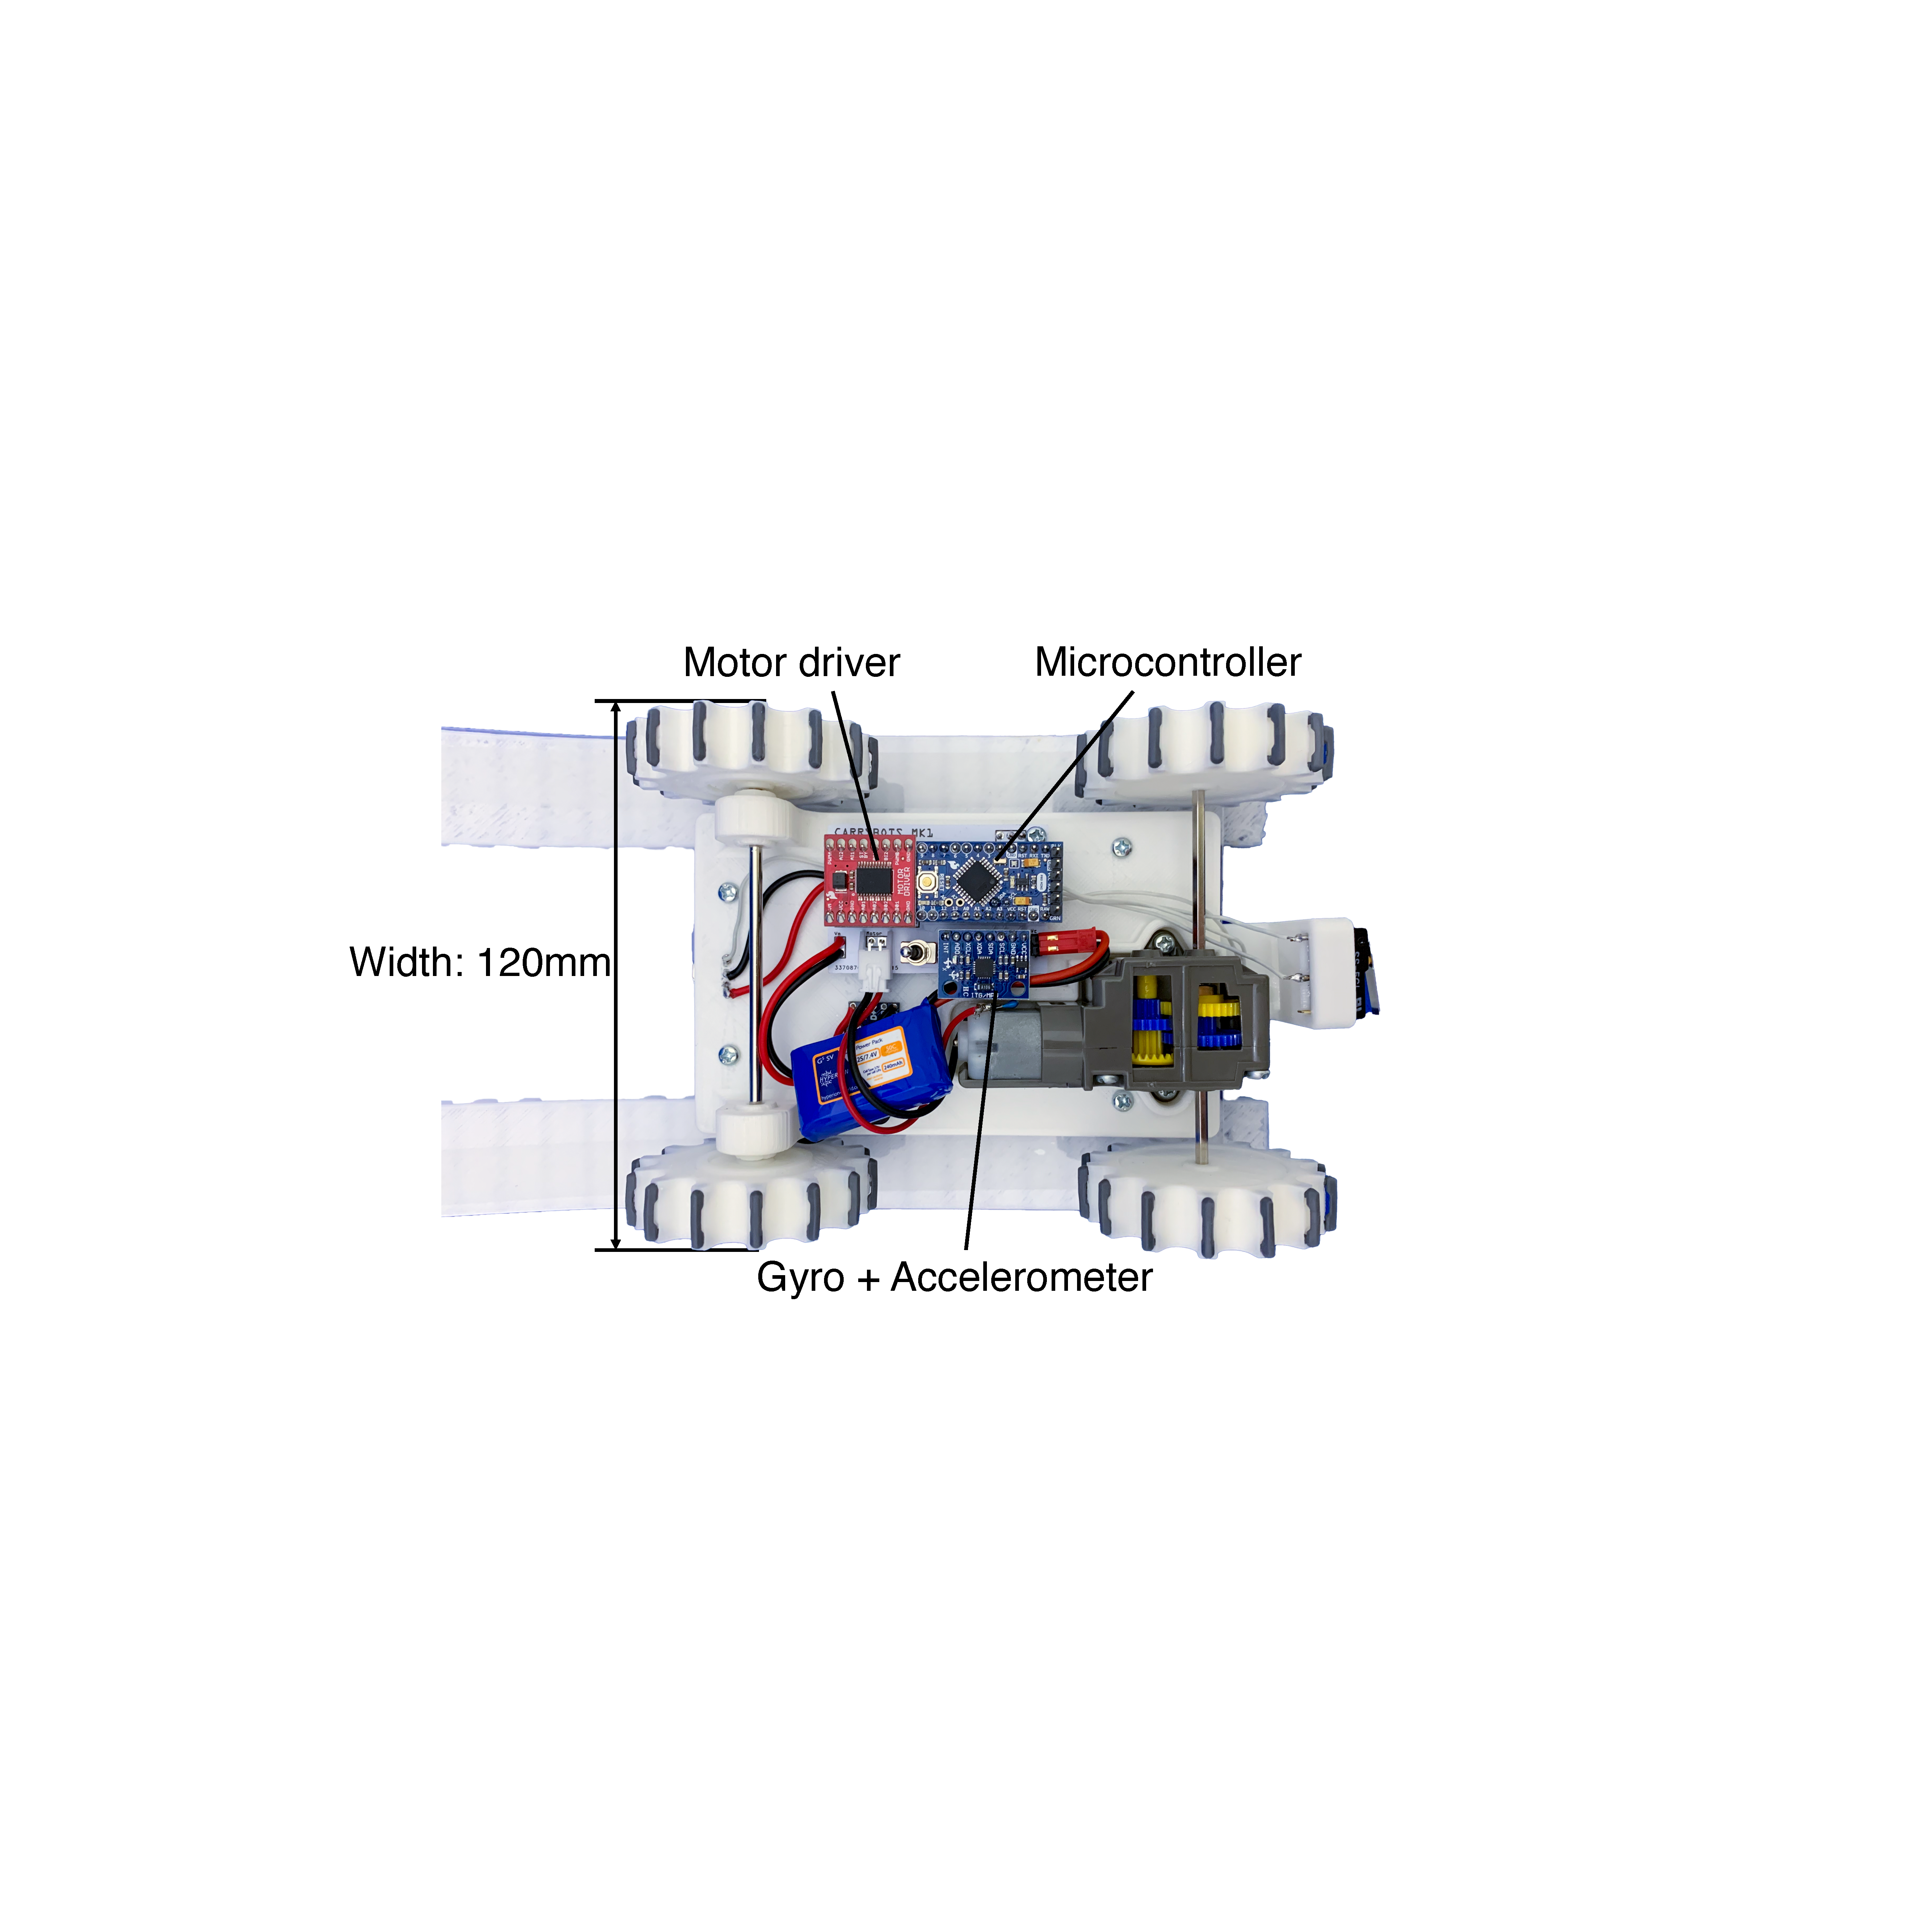
\includegraphics[width=\columnwidth]{figure/carrybot-bottom.pdf}
      \subcaption{Bottom view}
      \labfig{bottom-view}
    \end{minipage}
  \end{tabular}
  \centering
  \caption{Mechanical structure of the developed robot}
  \labfig{carrybot}
\end{figure}


\begin{table}[]
\caption{Specification of the robot}
\centering
\begin{tabular}{ll}
\hline
Weight & 306 g  \\
Width  & 120 mm \\
Length & 250 mm \\
Height & 70 mm  \\ \hline
\end{tabular}
\label{tab:robot-specs}
\end{table}

\begin{figure}[ht]
  \vspace{-9mm}
  \centering
  \begin{tabular}{c}
    \begin{minipage}[ht]{0.4\columnwidth}
      \centering
      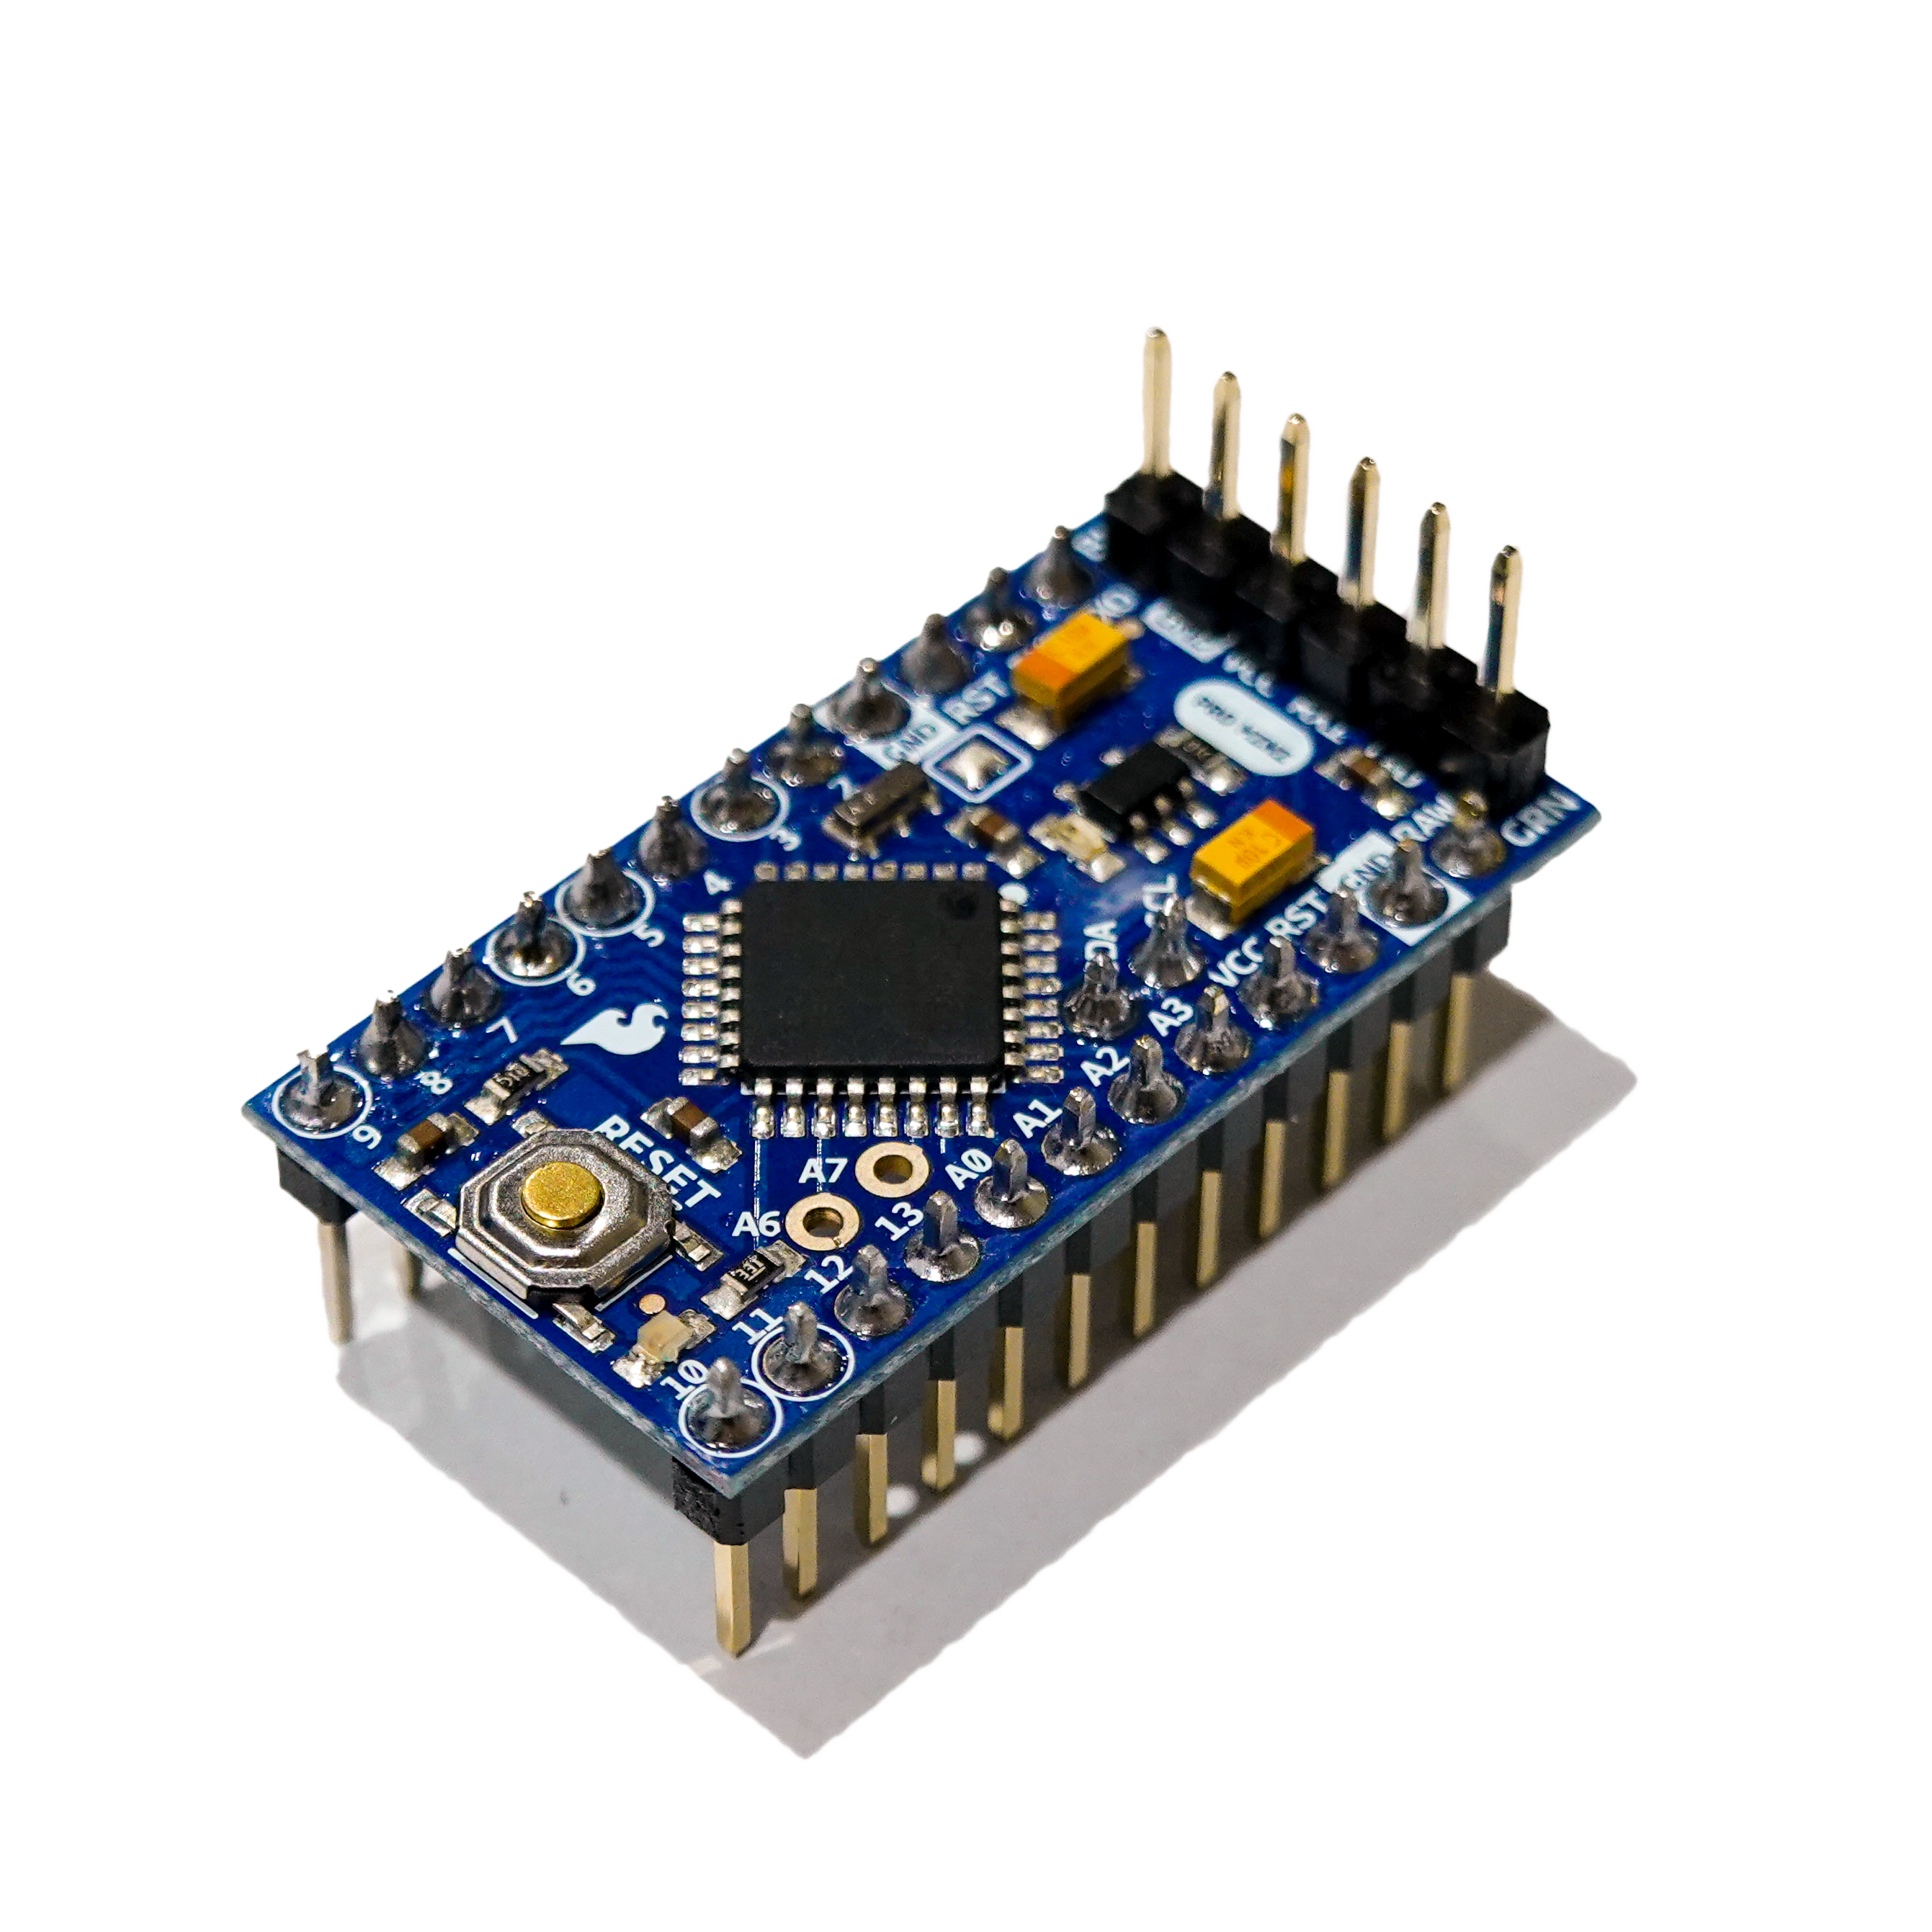
\includegraphics[trim=0 150 0 150, clip,width=0.8\columnwidth]{figure/arduino-pro-mini.png}
      \subcaption{Microcontroller}
      \labfig{arduino}
    \end{minipage}
    \begin{minipage}[ht]{0.4\columnwidth}
      \centering
      \includegraphics[trim=0 150 0 150, clip,width=0.8\columnwidth]{figure/lipo-battery.png}
      \subcaption{LiPo battery}
      \labfig{lipo}
    \end{minipage}\\
    
    \begin{minipage}[ht]{0.4\columnwidth}
      \centering
      \includegraphics[trim=0 150 0 150, clip,width=0.8\columnwidth]{figure/motor-driver.png}
      \subcaption{Motor driver}
      \labfig{motor-driver}
    \end{minipage}
    \begin{minipage}[ht]{0.4\columnwidth}
      \centering
      \includegraphics[trim=0 150 0 150, clip,width=0.8\columnwidth]{figure/DC-motor.png}
      \subcaption{Motor}
      \labfig{motor}
    \end{minipage}\\
    
    \begin{minipage}[ht]{0.4\columnwidth}
      \centering
      \includegraphics[trim=0 150 0 150, clip,width=0.8\columnwidth]{figure/limit-switch.png}
      \subcaption{Limit switch}
      \labfig{limit-switch}
    \end{minipage}
    \begin{minipage}[ht]{0.4\columnwidth}
      \centering
      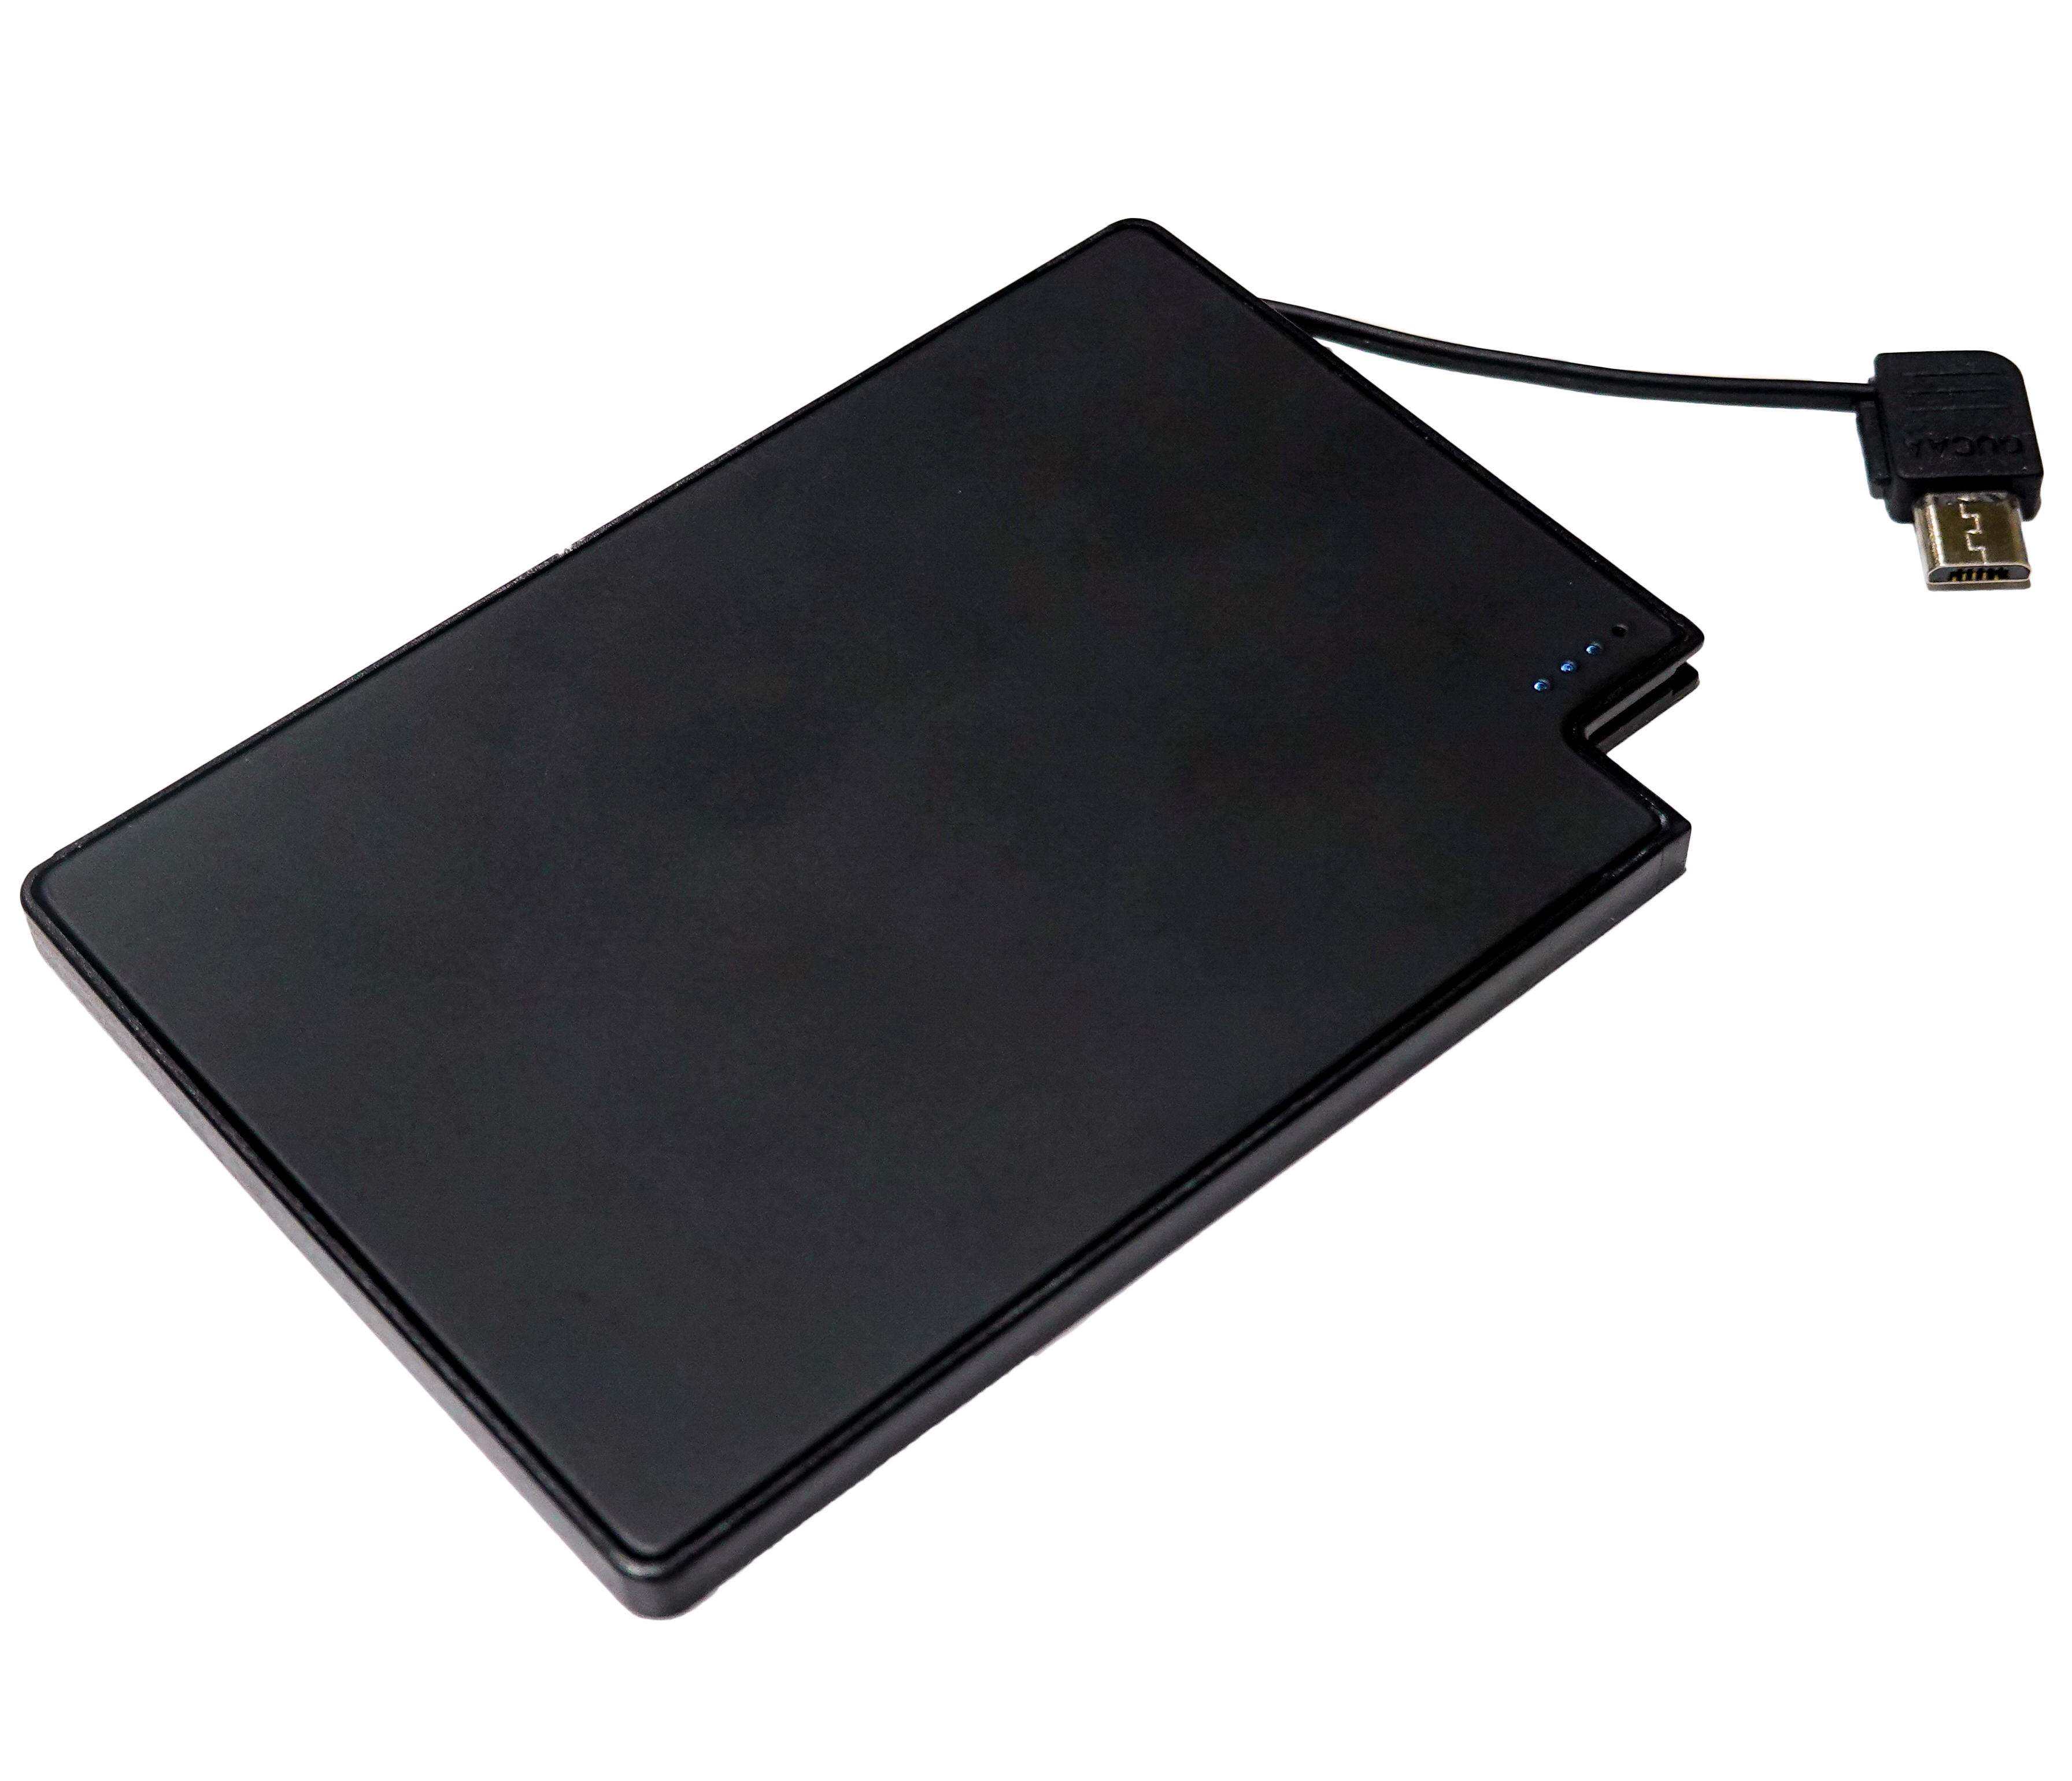
\includegraphics[width=0.8\columnwidth]{figure/mobile-battery.png}
      \subcaption{Power bank}
      \labfig{mobile-battery}
    \end{minipage}\\
    
        \begin{minipage}[ht]{0.4\columnwidth}
      \centering
      \includegraphics[trim=0 150 0 150, clip,width=.8\columnwidth]{figure/mpu6050.png}
      \subcaption{Gyro + Accelerometer}
      \labfig{mpu6050}
    \end{minipage}
    \begin{minipage}[ht]{0.4\columnwidth}
      \centering
      \includegraphics[trim=0 150 0 150, clip,width=.8\columnwidth]{figure/IR-receiver.png}
      \subcaption{IR receiver}
      \labfig{ir-receiver}
    \end{minipage}\\
    
  \end{tabular}
  \centering
  \caption{Overview of experimental instruments}
  \labfig{parts}
\end{figure}

\begin{itemize}
    \item マイコン(Arduino Pro Mini 328 5V 16MHz,SparkFun製) 1個
    \item モータドライバ(Motor Driver-Dual TB6612FNG(1A),SparkFun製) 1個
    \item モータ(FA-130タイプモータ,TAMIYA製)1個
    \item リミットスイッチ(超小型基本スイッチ SS-5GL,オムロン製)2個
    \item 6軸加速度センサージャイロセンサーモジュール(MPU-6050,HiLetgo製)1個
    \item 赤外線リモコン受信モジュール(OSRB38C9AA,OptoSupply製)1個
    \item リチウムイオンポリマー電池(G5 2S 240mAh LiPo 25C(4.2V),Hyperion製) 1個
    \item リチウムイオンポリマー電池(WT-H230 2500mAh(5V),Shenzhen LDTEK Technology Co., Ltd製)1個
\end{itemize}

Arduinoの電源は,リチウムイオンポリマー電池(7.4V)をArduinoに接続し,安定化回路で5Vを得ている.そして,モータの電源はモバイルバッテリー(5V)を使用し,マイクロUSBインターフェイスボード(CJMCU)を通して,給電する.また,赤外線リモコンからの信号を受信しやすくするため,赤外線リモコン受信モジュールを上に向けて,取り付ける.グリップ力を大きくするため,ピニオン車輪の歯先にTAMIYA製の脱着式の軟質樹脂製パッドを取り付ける.

モータはTAMIYA製のシングルギヤボックス(4速タイプ)を用いて,回転速度を$114.7:1$に減速している.モータは1つだけ用いており,左右のクローラーを同じ出力軸に繋ぐことで同量回転させて直進を実現している.ロボットが乗り上げるために,ロボットの後部のプラバンを鉛直下向きに垂れ下がるように曲げ,それをスペーサで挟み,ロボットに取り付ける.また,その上に,ラックレールを両面テープで固定する.これにより,後ろからきた他のロボットのピニオン車輪がラックレールとかみ合わさることで,乗り上げることができる.


\chapter{CarryBotsによる実機実験}
本章では,前章で製作したロボットを用いて行った実験について述べる.まず,乗り上げる動作の検証実験を行った.
% \begin{enumerate}
%     \item 乗り上げる動作の検証
% \end{enumerate}
% を行った.
その後,~\ref{section:modeling}で述べた物体をより安定に支持するための条件1,2を検証するために,ロボットと物体の高さの比を設計し,段数の変更による物体の安定化性能の検証実験と,ロボットに前進力をかけて,制御による物体の安定化性能の検証実験を行った.
% \begin{enumerate}
%     \setcounter{enumi}{1}
%     \item 段数の変更による物体の安定化性能の検証
%     \item 制御による物体の安定化性能の検証
% \end{enumerate}
% に関する実験を行った.
そして,それぞれの検証で得られた結果と,それらに対する考察を述べる.
% そして,ロボット1とロボット2の前進力の差$F_{r_{1}}-F_{r_{2}}$を大きくすることに着目し,
% \begin{enumerate}
%     \setcounter{enumi}{2}
%     \item 制御による物体の安定化性能の検証
% \end{enumerate}
% に関する実験を行った.
%%%%%%%%%%%%%%%%%%%%%%%%%%%%%%%%%%%%%%%%%%%%%%%%%%%%%%%%%%%%%%%%%%%%%%%%%

\section{乗り上げる動作の検証}
前章で製作したロボットが他のロボットに乗り上げることが実現できるかどうかを実機検証した.

\subsection{実験手順}
搬送物体として本を平坦な床に立てて置き,その左側に製作したロボットと同じ程度のTAMIYA製のキャタピラ車を2台重ねて置いた.物体の右側には1列縦隊で製作したロボットを左向きに4台間隔をあけ並べて配置した.そして1台目のロボットにリモコンを用いて前進の指令を与えた.ロボットが本に近づいたら,リモコンで停止の指令を与えた.これを3回繰り返して,ロボットが乗り上げる様子を撮影した.

\subsection{実験結果}
4台のロボットによる3段までの乗り上げる様子を\reffig{climb}に示す.ロボットAは本に近づいて,止まった.そして,ロボットBがロボットAに乗り上げ,本の前に止まった.続いて,ロボットCがロボットBの後ろに止まった.その後,ロボットDがロボットB・Cに乗り上げ,3段まで乗り上げられることが確認できた.

\begin{figure}[tb]
  \centering
  \includegraphics[width=\columnwidth]{figure/climb.pdf}
  \caption{Experiment of climbing over each other}
  \label{fig:climb}
\end{figure}

\subsection{考察}
このピニオン車輪とラックレール機構を使うと,ロボットが乗り上げる際に,ピニオン車輪は空転することや,滑ることがなく,安定に乗り上げられることが確認できた.また,一般に使われている車輪やクローラーより効率よく,安定に乗り上げることも言える.
そして,ロボットが乗り上げる際,前方のロボットを動かさずに乗り上げることができるので,前のロボットが物体を支持しているときでも,物体に影響を与えず,乗り上げられると言える.
その他,最初にピニオン車輪とラックレールがかみ合わなくても,車輪が回し続けると,自重で受動的にかみ合うことがわかった.よって,ロボットが1列縦隊であれば,どのような場合でもピニオン車輪をラックレールとかみ合わせられると言える.
%%%%%%%%%%%%%%%%%%%%%%%%%%%%%%%%%%%%%%%%%%%%%%%%%%%%%%%%%%%%%%%%%%%%%%%%%

\section*{牽引装置}
乗り上げることを確認できた後,物体の安定化性能に関する実験を行った.つまり,移動ロボットが移動しているとき,支持部のロボットが物体を支持できるかどうかを確認する.ここからの実験は提案システムの移動部をロボットの代わりとして,紙を使用した.また,紙を一定力で引っ張るために,\reffig{pulling-mechanism-concept}に示すような牽引装置を作製した.牽引装置はTAMIYA社のキャタピラ車をワイヤで机に前進しないように固定し,安定化電源で一定の電圧をかける.このとき,クローラーが摩擦よって,紙を巻き取り,紙の上に載せているものを一定速度で動かすことができる.また,\reffig{pulling-mechanism}に示すように,クローラーと紙の間の摩擦を上げるために,グリップ力の高いの脱着式の軟質樹脂製パッドのついている連結式クローラーを利用した.そして,接触面積を大きくするために,クローラーをひっくり返し,さらにクローラーと紙の間の摩擦を大きくするために,クローラー車の上に巻きはんだを載せておもりとして利用した.
\begin{figure}[b]
  \centering
  \includegraphics[width=0.75\columnwidth]{figure/concept-pulling-mechanism.pdf}
  \caption{Concept of pulling mechanism}
  \label{fig:pulling-mechanism-concept}
\end{figure}
\begin{figure}[tb]
  \centering
  \includegraphics[width=0.7\columnwidth]{figure/pulling-mechanism-v2.pdf}
  \caption{Pulling mechanism}
  \label{fig:pulling-mechanism}
\end{figure}

また,物体の姿勢を評価するために,\reffig{gopro}に示すように,紙の上にカメラ(GoPro Hero 3 Black)を固定した.これによってカメラを搬送物体と同じ速度で動かすことができ,トラッキングによって物体の角度を計測することが可能である.

\begin{figure}[tb]
  \centering
  \includegraphics[width=0.7\columnwidth]{figure/gopro.pdf}
  \caption{Camera for tracking the angle of object}
  \label{fig:gopro}
\end{figure}
この牽引装置を利用して,以下の実験を行った.

\section{段数の変更による物体の安定化性能に関する実験}
\label{section:exp2}
~\ref{section:modeling}で述べたロボットと物体の高さの比$\frac{h_{r}}{h_{o}}$を大きくすることにより物体をより安定に支持することを検証するために,
製作したロボットを積み重ねることで,物体を支持することが可能であるかの検証を行った.さらに全体の加速度と物体の角度の解析を行った.

\subsection{実験手順}
上で述べた紙の上に,搬送物体として本を立てて置いた.その両側にロボットを1段ずつと2段ずつ置き,牽引装置に6Vの電圧を印加したときの安定化性能の比較を行った.

\subsection{実験結果と考察}
まず,物体の両側にロボットを1段および2段置いた場合の実験の様子を\reffig{exp-layers}に示す.また,そのときの全体の加速度の変化と物体の角度の変化を\reffig{acc-1v2}と\reffig{angle-1v2}にそれぞれ示す.
\begin{figure}[tb]
  \vspace{0mm}
  \centering
  \begin{tabular}{c}
    \begin{minipage}[ht]{0.5\columnwidth}
      \centering
      \includegraphics[width=\columnwidth]{figure/1layer.pdf}
      \subcaption{1 layer}
      \labfig{6v-1layer}
    \end{minipage}
    \begin{minipage}[ht]{0.5\columnwidth}
      \centering
      \includegraphics[width=\columnwidth]{figure/2layers.pdf}
      \subcaption{2 layers}
      \labfig{6v-2layer}
    \end{minipage}
  \end{tabular}
  \centering
  \caption{Experiment of changing supporting layers}
  \labfig{exp-layers}
\end{figure}

\reffig{6v-1layer}より,ロボットが1段の場合では紙を引っ張り出すと,物体はすぐ倒れた.一方,\reffig{6v-2layer}より,ロボットが2段の場合では紙を引っ張り出してから止まるまで物体は最初の姿勢を保つことができた.
\begin{figure}[tb]
 \centering
  \begin{tabular}{c}
   
   \begin{minipage}{\hsize}
    \centering
     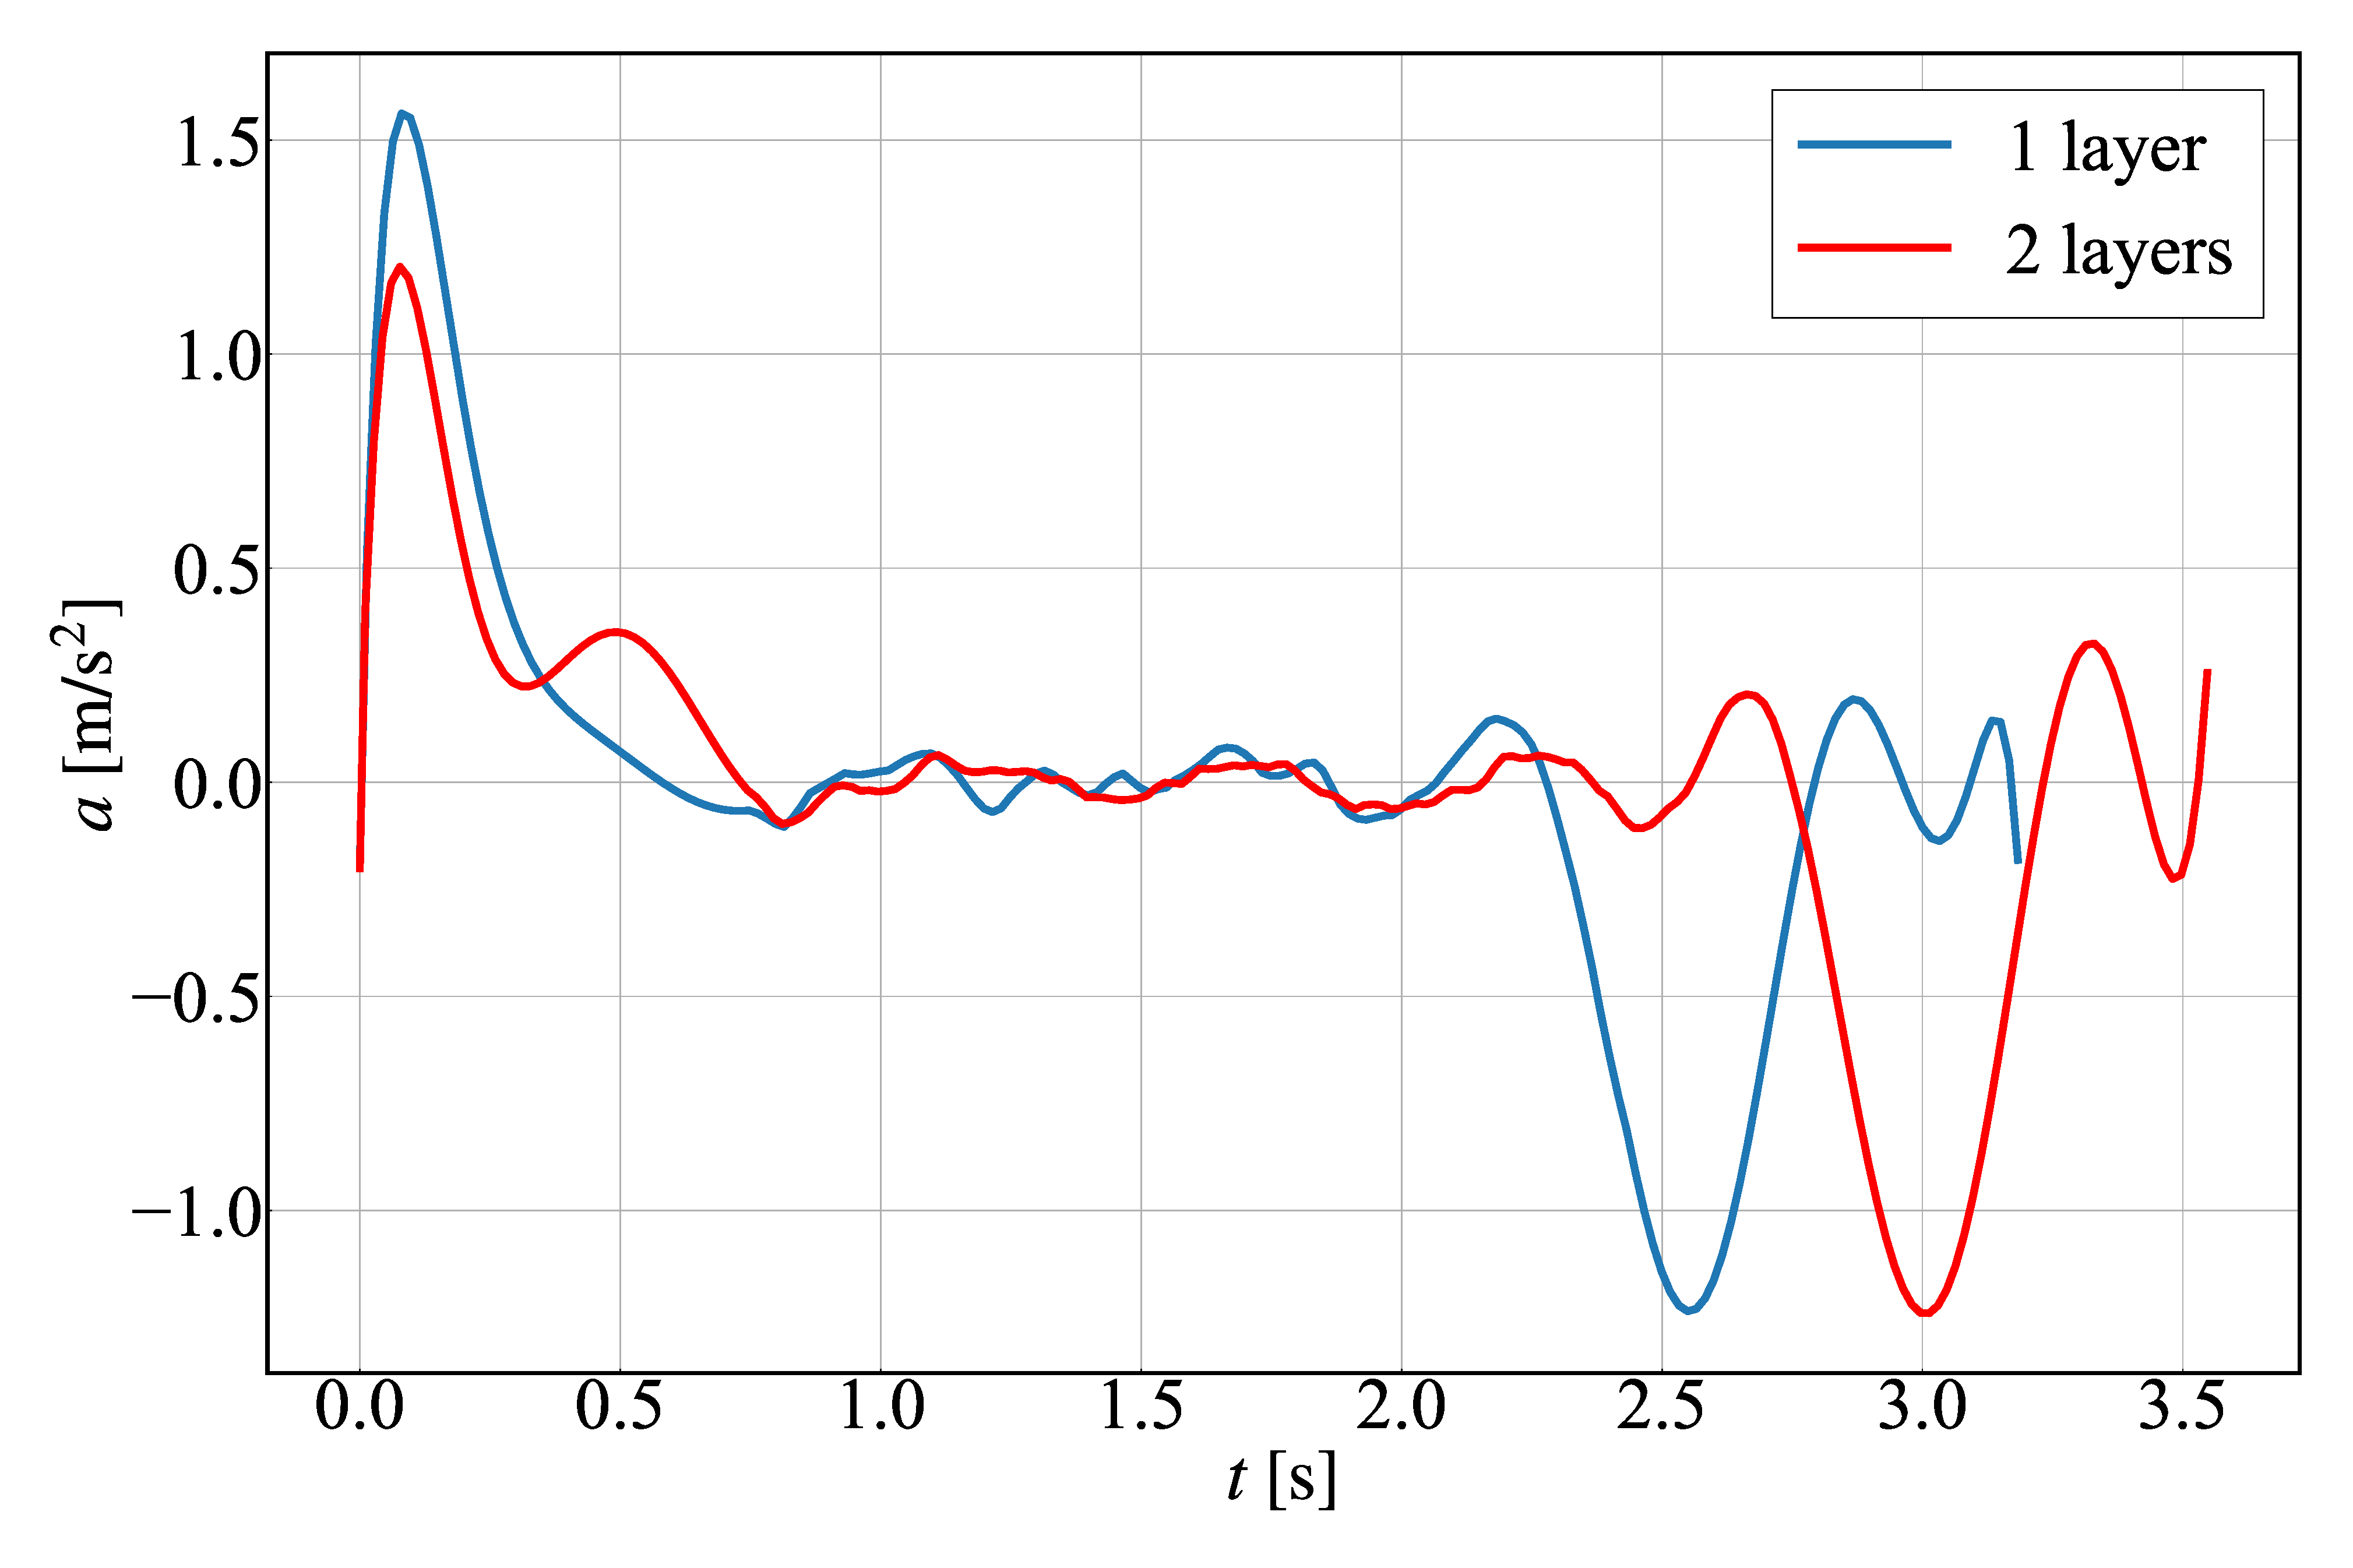
\includegraphics[width=0.63\columnwidth, angle=0]{figure/acc-graph-1v2.eps}
     \caption{Change in acceleration(Layer)}
     \labfig{acc-1v2}
   \end{minipage}\\
   
   \begin{minipage}{\hsize}
    \centering
     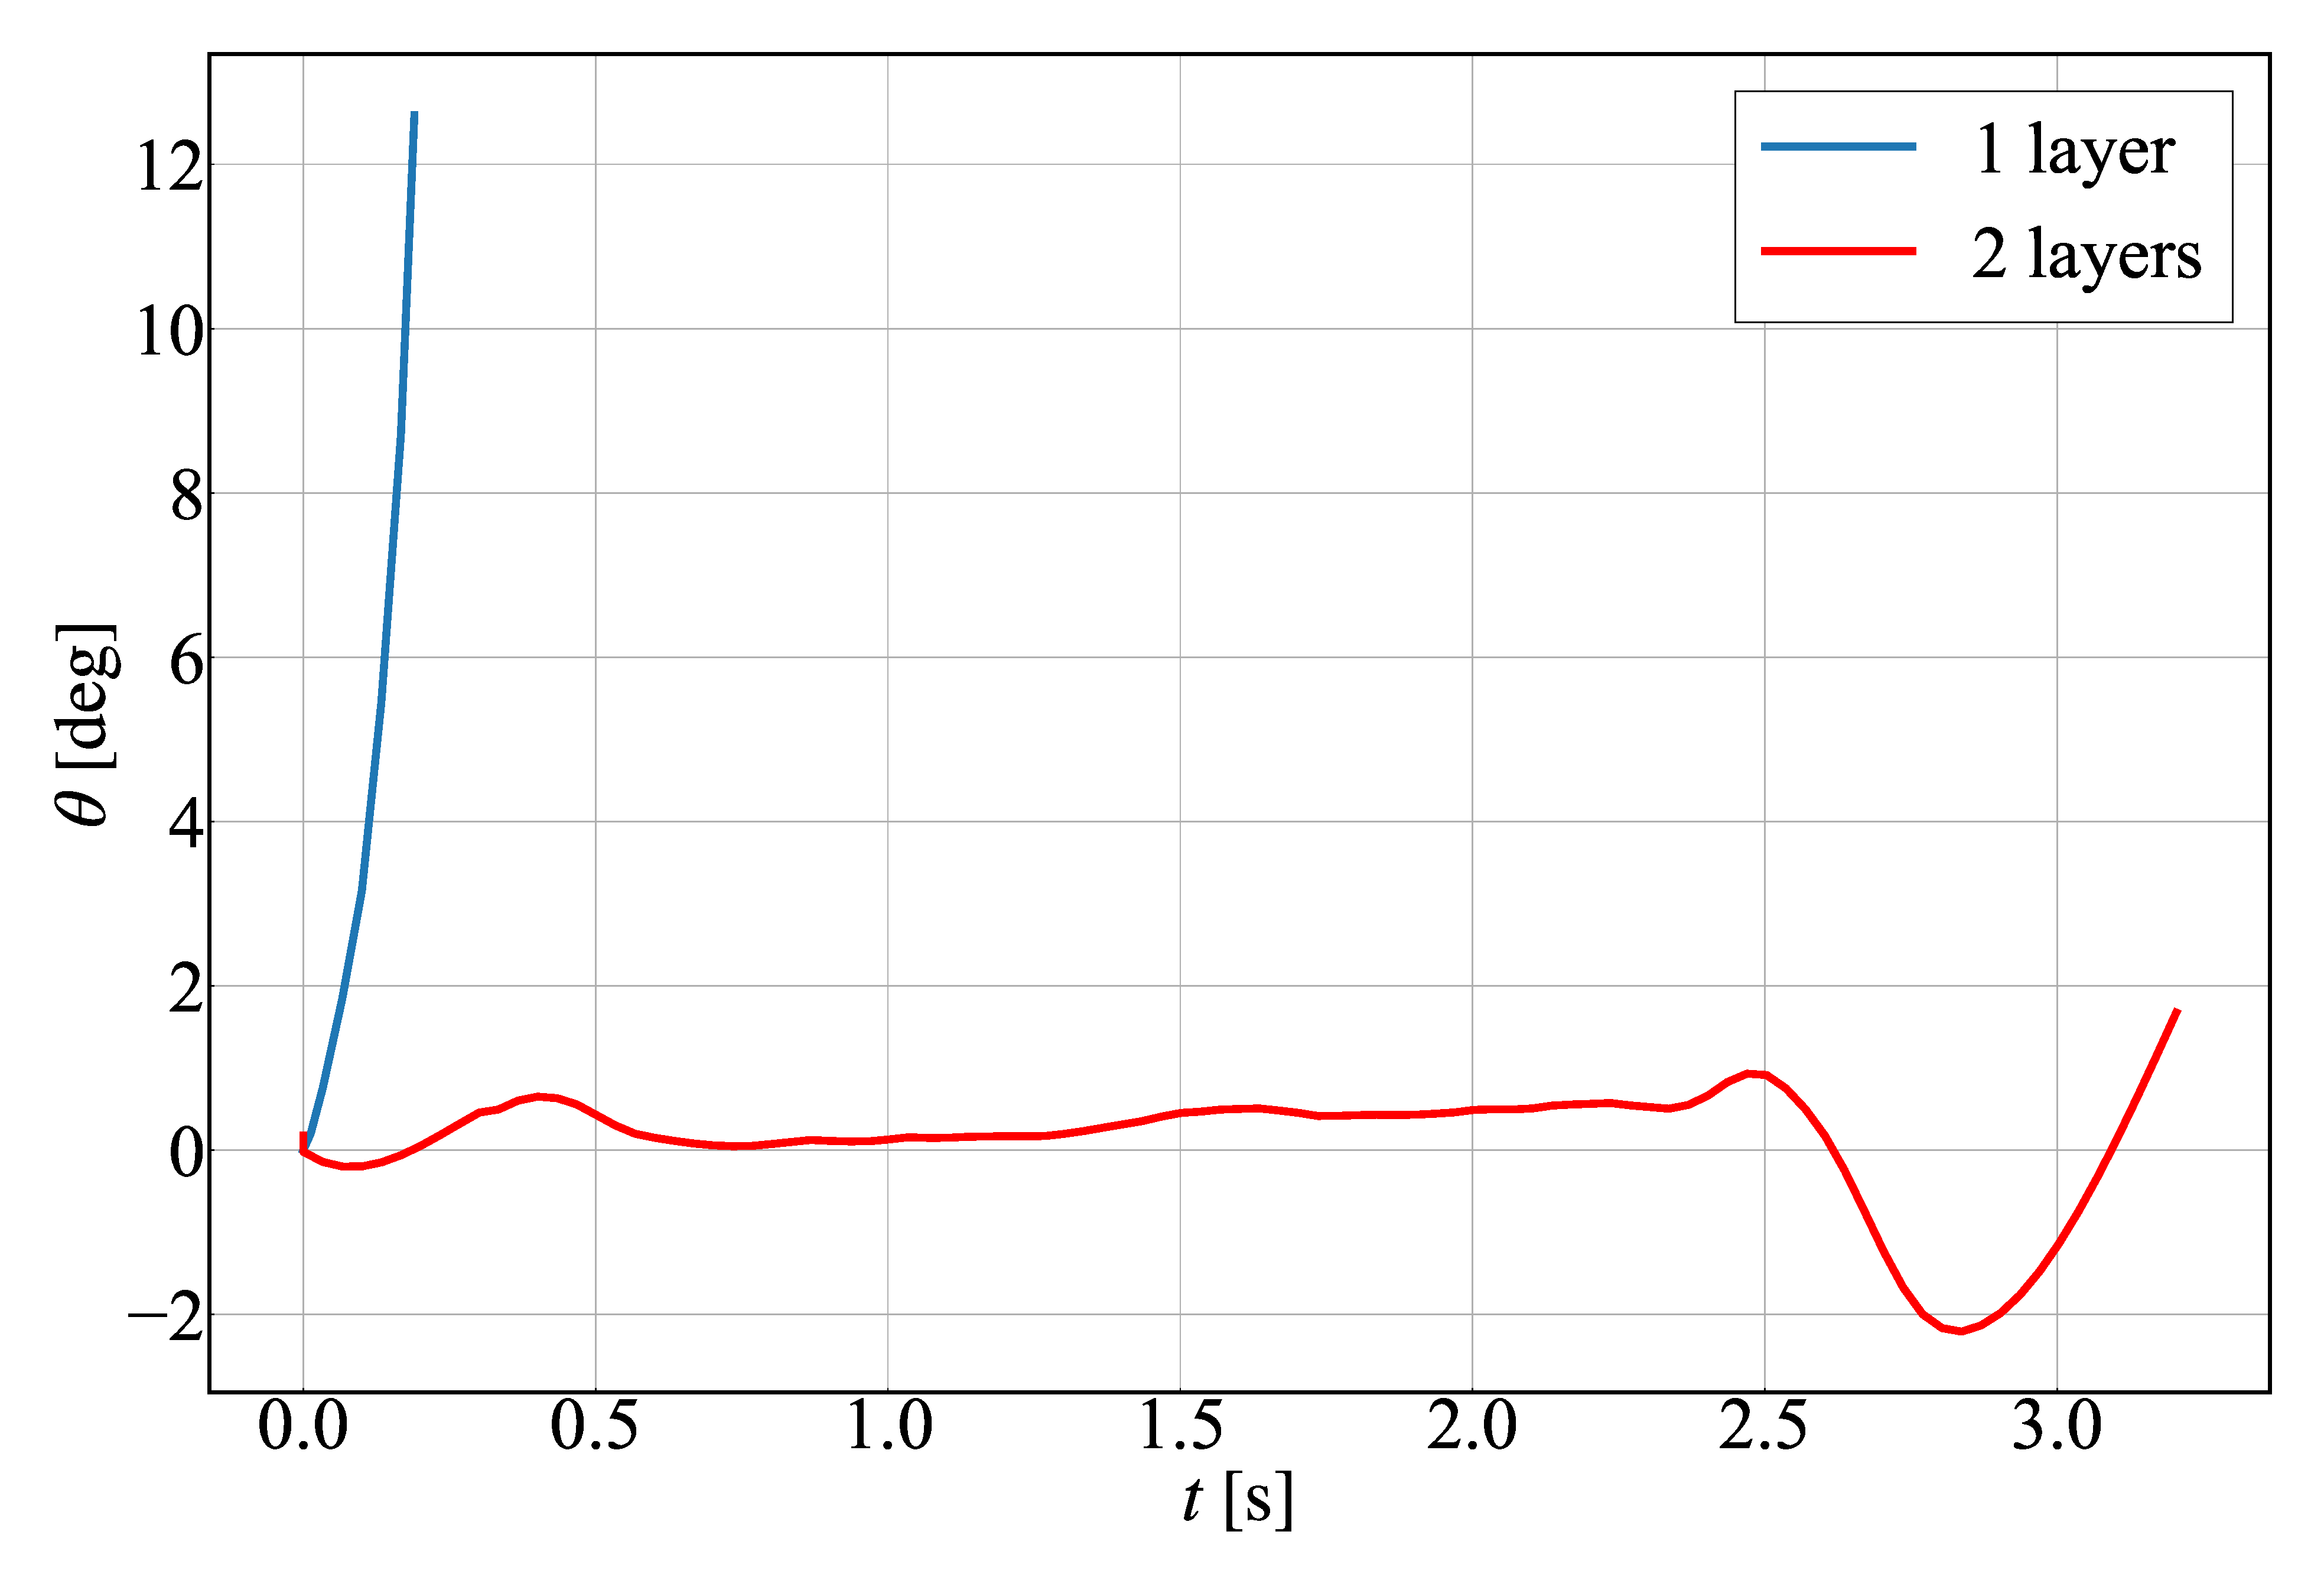
\includegraphics[width=0.6\columnwidth, angle=0]{figure/angle-1vs2.eps}
     \caption{Change in angle(Layer)}
     \labfig{angle-1v2}
   \end{minipage}
  \end{tabular}
\end{figure}

そして,\reffig{acc-1v2}では,横軸は時間,縦軸は紙の動く加速度である.\reffig{acc-1v2}より,牽引装置に電圧を印加する瞬間,つまり時刻が$t=0$~sから$t=0.5$~sの間では1段と2段の場合とも加速されていることがわかった.そのとき,1段の場合の全体の最大加速度は$a_{max}=1.5$~\si{m/s^2}であったが,2段の場合は$a_{max}=1.3$~\si{m/s^2}であった.その原因は2段に積むと,支持部全体の質量は1段の方より大きいので,紙と机の間の摩擦は1段より大きいと考えられる.
$t=0.5$~sから$t=2.3$~sの間では加速度は0~\si{m/s^2}付近であり,等速で移動することが確認できた.その後,牽引装置の印加電圧を遮断すると,全体が減速し,止まった.
次に,\reffig{angle-1v2}では,横軸は時間,縦軸は物体の初期姿勢からの角度のずれである.ここで,物体の角度は進行方向の逆向きを正とする.1段の場合の角度は設定された$\pm5$\si{\degree}範囲外にあることがわかった.一方2段の場合は動き出してから,減速までの間で$-0.3$\si{\degree}$\sim0.9$\si{\degree}に収まることが確認できた.
この結果より,牽引装置の印加電圧が6Vのとき,全体の加速度が大きいため,1段で支持する場合はロボットが滑ってしまい,物体を支持できなくなる.しかし,2段に増やすと,物体の重心近くで支持することと,2段のロボットが紙から滑りにくくなることによって,物体を支持し,移動することができると考えられる.

\section{制御による物体の安定化性能に関する実験}
\label{section:exp3}
~\ref{section:modeling}で述べたロボット1とロボット2の前進力$F_{r_{1}}$,$F_{r_{2}}$を加えることにより物体をより安定に支持することを検証するために,
製作したロボットの物体の姿勢を検知するセンサを利用し,物体の初期姿勢に戻そうとする制御をかけると,前節では物体を支持することができなかったロボットが1段の場合でも,物体を支持できるかを確認する実験を行った.さらに全体の加速度と物体の角度の解析を行った.

\subsection{実験手順}
まず,かける制御について述べる.それを\reffig{overview-control}に示す.\reffig{upright}より,物体の姿勢を検知するセンサの上下両方のスイッチが反応したとき,ロボットに対して物体は安定であると判断し,ロボットは前進しない.
しかし,\reffig{tilt}より,もし物体が右に傾いている場合,左のロボットに取り付けられた物体の姿勢を検知するセンサは下のスイッチのみ反応するが,一方,右のロボットに取り付けられたセンサは上のスイッチのみ反応する.このとき,右のロボットが左のロボットより大きい速度で物体を押し付けることで,物体の姿勢を保つと考える.
\begin{figure}[tb]
 \centering
  \begin{tabular}{c}
   
   \begin{minipage}{\hsize}
    \centering
    \includegraphics[width=0.8\columnwidth]{figure/control-upright.pdf}
      \subcaption{Object is upright}
      \label{fig:upright}
   \end{minipage}\\
   
   \begin{minipage}{\hsize}
    \centering
    \includegraphics[width=0.8\columnwidth]{figure/control-tilted-v2.pdf}
      \subcaption{Object is tilted}
      \label{fig:tilt}
   \end{minipage}
  \end{tabular}
  \caption{Overview of control system}
  \label{fig:overview-control}
\end{figure}

~\ref{section:exp2}で述べた実験と同じく,ロボットを物体の両側に置いて,牽引装置に6Vの電圧を印加した場合について,安定化性能の比較を行った.

\subsection{実験結果と考察}
まず,物体の姿勢を検知するセンサによって制御をかけた場合の実験の様子を\reffig{control}に示す.また,そのときの全体の加速度の変化と物体の角度の変化を\reffig{acc-1vC}と\reffig{angle-1vC}にそれぞれを示す.
\begin{figure}[tb]
  \centering
  \includegraphics[width=0.6\columnwidth]{figure/control.pdf}
  \caption{Experiment of applying control}
  \label{fig:control}
\end{figure}

\reffig{control}より,紙を引っ張り出した瞬間,ロボットはまだ反応していないときに,物体は傾いた.しかし,その後はロボットのセンサが反応するため,ロボットが物体を初期姿勢に戻そうとする.これによって全体が止まるまで物体を支持できることが確認できた.

\begin{figure}[tb]
 \centering
  \begin{tabular}{c}
   
   \begin{minipage}{\hsize}
    \centering
     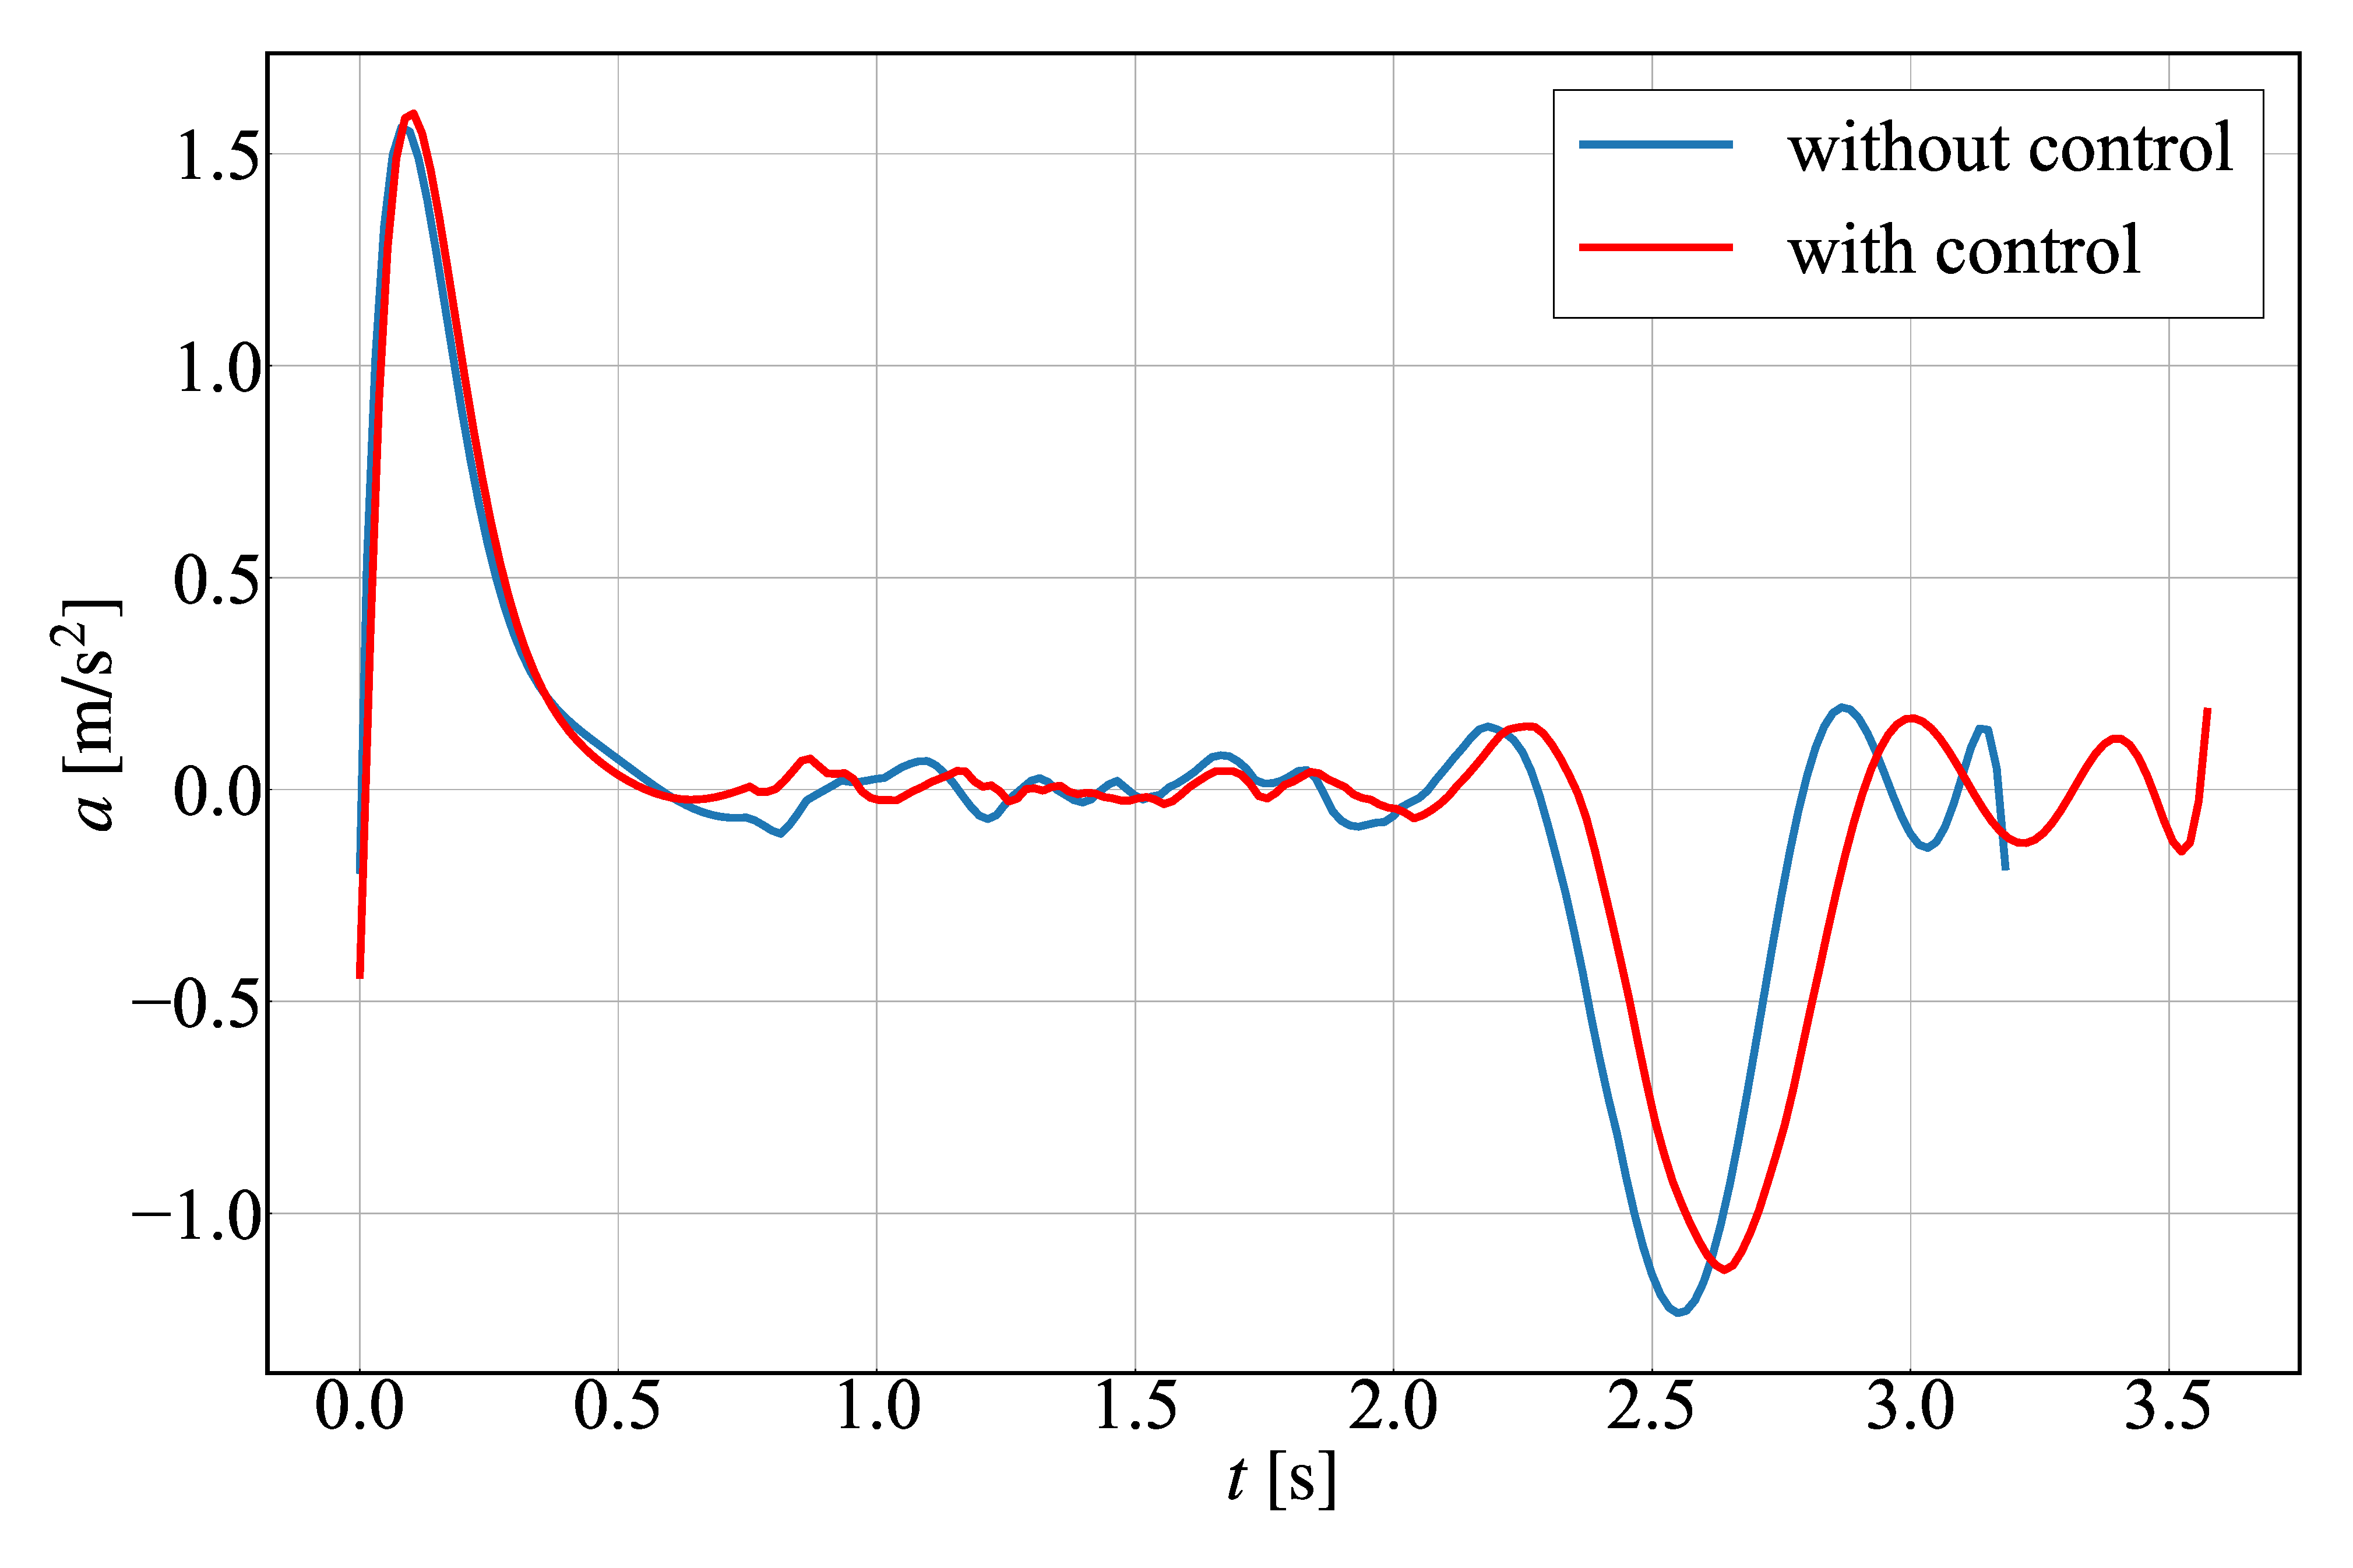
\includegraphics[width=0.63\columnwidth]{figure/acc-graph-control.eps}
     \caption{Change in acceleration(Control)}
     \labfig{acc-1vC}
   \end{minipage}\\
   
   \begin{minipage}{\hsize}
    \centering
     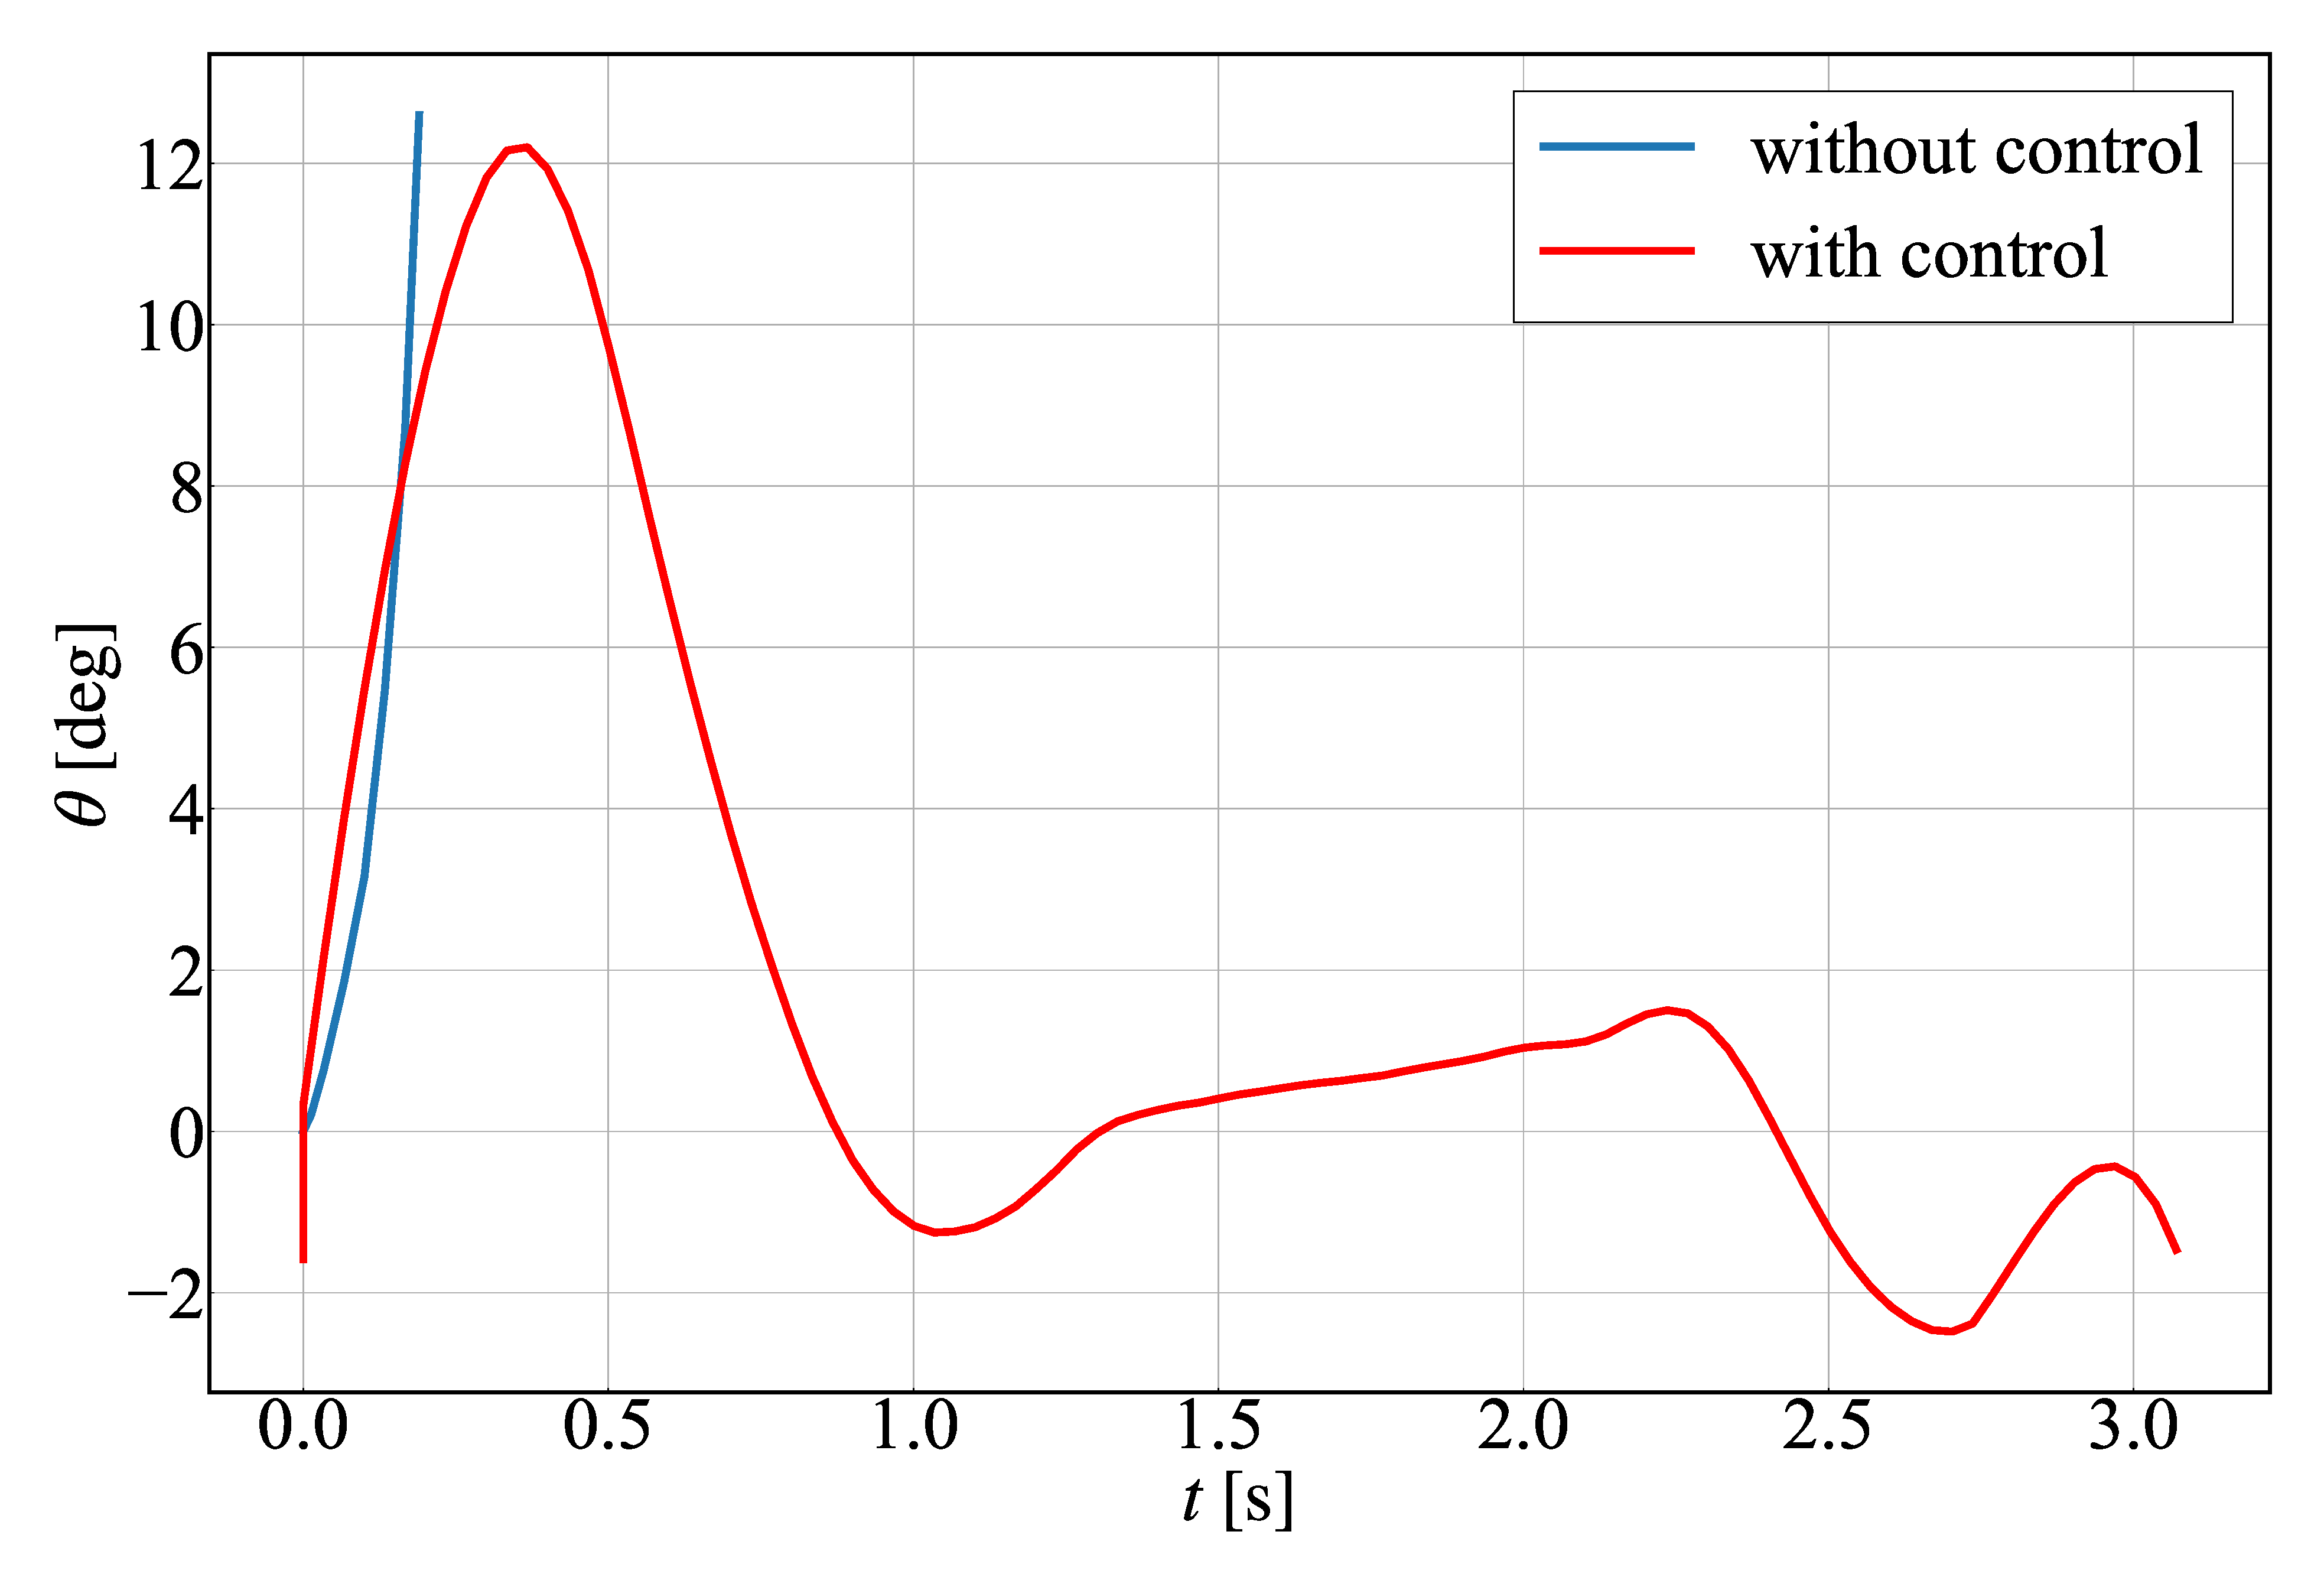
\includegraphics[width=0.6\columnwidth]{figure/angle-control.eps}
     \caption{Change in angle(Control)}
     \labfig{angle-1vC}
   \end{minipage}
  \end{tabular}
\end{figure}
そして,\reffig{acc-1vC}では,横軸は時間,縦軸は紙の動く加速度である.\reffig{acc-1vC}より,牽引装置に電圧を印加する瞬間,つまり時刻が$t=0$~sから$t=0.5$~sの間では制御なしと制御ありの場合両方とも同じ加速度で加速されていることがわかった.牽引装置に同じ電圧を印加し,支持部のロボットの台数も同じなので,加速度が一致していることは妥当である.
また,$t=0.5$~sから$t=2.3$~sの間では加速度は0~\si{m/s^2}付近であるので,等速で移動することが確認できた.その後,牽引装置の印加電圧を遮断すると,全体が減速し,止まることが確認できた.
次に,\reffig{angle-1vC}では,横軸は時間,縦軸は物体の初期姿勢からの角度のずれである.ここで,~\ref{section:exp2}の実験と同じく物体の角度は進行方向の逆向きを正とする.制御なしの場合の角度は設定された$\pm5$\si{\degree}範囲外にあることがわかった.一方,制御ありの場合は,$t=0$~sから$t=0.5$~sまでは,物体の初期姿勢から12\si{\degree}傾いたものの,$t=0.5$~s以降,物体の初期姿勢からの角度差は0に収束し,$\pm1.8$\si{\degree}範囲内に振動することがわかった.
よって,制御をかけることで,ロボット1段でも支持することができると言える.その他,急に動き出すときの大きい角度差に対して,今後ロボットに搭載されている加速度センサを利用して,フィードフォワード制御をかけることで,より安定に運搬できると考えられる.
\chapter{結言}
本研究の目的は不安定物体に応じて安定性と機動性を両立した協調運搬可能な群ロボットの開発である.
その前段階として,本論文では,システムの支持部が物体を支えるための条件を検討し,システムのモデリングをした上で,物体が傾けるときの条件を調べた.また,モデリングした式から,ロボットの間の摩擦を上げることで,より安定な支持・運搬作業ができることがわかった.そのほか,それを実現可能な群ロボットシステムを開発した.
そして,実機実験を行い,提案システムの妥当性が確認できた.実験結果より,ロボットが他のロボットに乗り上げられること,移動部が移動するとき不安定な物体を支持できることが確認できた.また,制御することで,より安定な協調運搬も確認できた.
今後の研究としては,まず,移動部のロボット同士をつなげる機構を考え,移動部を紙からロボットに変える.また,移動部と支持部の最適な割合の設計も考えて行きたい.最後に,ロボットの体を生かして,自身で溝を埋めて地面になったり,結合して橋になったりして仲間を渡らせたりすることができる群ロボットシステムにもつなげて行きたい.



%謝辞
\chapter*{謝辞}
本論文をまとめるにあたり,数多くの御助言,御提案,活発な議論をしていただいた大須賀公一教授,杉本靖博准教授,末岡裕一郎助教に心から感謝申し上げます.
また研究を進める際に,Swarmチームをはじめ,大須賀・杉本研究室の皆様には数多くの御助言,御協力をいただきましたことを深く感謝いたします.

%参考文献
%参考文献
\bibliographystyle{osukalab}
\bibliography{bibtex/ref}


\appendix
%付録
%\chapter{}
%\input{contents/7.appendix}

\end{document}
